% Options for packages loaded elsewhere
\PassOptionsToPackage{unicode}{hyperref}
\PassOptionsToPackage{hyphens}{url}
%
\documentclass[
]{book}
\usepackage{lmodern}
\usepackage{amssymb,amsmath}
\usepackage{ifxetex,ifluatex}
\ifnum 0\ifxetex 1\fi\ifluatex 1\fi=0 % if pdftex
  \usepackage[T1]{fontenc}
  \usepackage[utf8]{inputenc}
  \usepackage{textcomp} % provide euro and other symbols
\else % if luatex or xetex
  \usepackage{unicode-math}
  \defaultfontfeatures{Scale=MatchLowercase}
  \defaultfontfeatures[\rmfamily]{Ligatures=TeX,Scale=1}
\fi
% Use upquote if available, for straight quotes in verbatim environments
\IfFileExists{upquote.sty}{\usepackage{upquote}}{}
\IfFileExists{microtype.sty}{% use microtype if available
  \usepackage[]{microtype}
  \UseMicrotypeSet[protrusion]{basicmath} % disable protrusion for tt fonts
}{}
\makeatletter
\@ifundefined{KOMAClassName}{% if non-KOMA class
  \IfFileExists{parskip.sty}{%
    \usepackage{parskip}
  }{% else
    \setlength{\parindent}{0pt}
    \setlength{\parskip}{6pt plus 2pt minus 1pt}}
}{% if KOMA class
  \KOMAoptions{parskip=half}}
\makeatother
\usepackage{xcolor}
\IfFileExists{xurl.sty}{\usepackage{xurl}}{} % add URL line breaks if available
\IfFileExists{bookmark.sty}{\usepackage{bookmark}}{\usepackage{hyperref}}
\hypersetup{
  pdftitle={Data Science Untuk Pemula},
  pdfauthor={Bakti Siregar S.Si, M.Sc},
  hidelinks,
  pdfcreator={LaTeX via pandoc}}
\urlstyle{same} % disable monospaced font for URLs
\usepackage{color}
\usepackage{fancyvrb}
\newcommand{\VerbBar}{|}
\newcommand{\VERB}{\Verb[commandchars=\\\{\}]}
\DefineVerbatimEnvironment{Highlighting}{Verbatim}{commandchars=\\\{\}}
% Add ',fontsize=\small' for more characters per line
\usepackage{framed}
\definecolor{shadecolor}{RGB}{248,248,248}
\newenvironment{Shaded}{\begin{snugshade}}{\end{snugshade}}
\newcommand{\AlertTok}[1]{\textcolor[rgb]{0.94,0.16,0.16}{#1}}
\newcommand{\AnnotationTok}[1]{\textcolor[rgb]{0.56,0.35,0.01}{\textbf{\textit{#1}}}}
\newcommand{\AttributeTok}[1]{\textcolor[rgb]{0.77,0.63,0.00}{#1}}
\newcommand{\BaseNTok}[1]{\textcolor[rgb]{0.00,0.00,0.81}{#1}}
\newcommand{\BuiltInTok}[1]{#1}
\newcommand{\CharTok}[1]{\textcolor[rgb]{0.31,0.60,0.02}{#1}}
\newcommand{\CommentTok}[1]{\textcolor[rgb]{0.56,0.35,0.01}{\textit{#1}}}
\newcommand{\CommentVarTok}[1]{\textcolor[rgb]{0.56,0.35,0.01}{\textbf{\textit{#1}}}}
\newcommand{\ConstantTok}[1]{\textcolor[rgb]{0.00,0.00,0.00}{#1}}
\newcommand{\ControlFlowTok}[1]{\textcolor[rgb]{0.13,0.29,0.53}{\textbf{#1}}}
\newcommand{\DataTypeTok}[1]{\textcolor[rgb]{0.13,0.29,0.53}{#1}}
\newcommand{\DecValTok}[1]{\textcolor[rgb]{0.00,0.00,0.81}{#1}}
\newcommand{\DocumentationTok}[1]{\textcolor[rgb]{0.56,0.35,0.01}{\textbf{\textit{#1}}}}
\newcommand{\ErrorTok}[1]{\textcolor[rgb]{0.64,0.00,0.00}{\textbf{#1}}}
\newcommand{\ExtensionTok}[1]{#1}
\newcommand{\FloatTok}[1]{\textcolor[rgb]{0.00,0.00,0.81}{#1}}
\newcommand{\FunctionTok}[1]{\textcolor[rgb]{0.00,0.00,0.00}{#1}}
\newcommand{\ImportTok}[1]{#1}
\newcommand{\InformationTok}[1]{\textcolor[rgb]{0.56,0.35,0.01}{\textbf{\textit{#1}}}}
\newcommand{\KeywordTok}[1]{\textcolor[rgb]{0.13,0.29,0.53}{\textbf{#1}}}
\newcommand{\NormalTok}[1]{#1}
\newcommand{\OperatorTok}[1]{\textcolor[rgb]{0.81,0.36,0.00}{\textbf{#1}}}
\newcommand{\OtherTok}[1]{\textcolor[rgb]{0.56,0.35,0.01}{#1}}
\newcommand{\PreprocessorTok}[1]{\textcolor[rgb]{0.56,0.35,0.01}{\textit{#1}}}
\newcommand{\RegionMarkerTok}[1]{#1}
\newcommand{\SpecialCharTok}[1]{\textcolor[rgb]{0.00,0.00,0.00}{#1}}
\newcommand{\SpecialStringTok}[1]{\textcolor[rgb]{0.31,0.60,0.02}{#1}}
\newcommand{\StringTok}[1]{\textcolor[rgb]{0.31,0.60,0.02}{#1}}
\newcommand{\VariableTok}[1]{\textcolor[rgb]{0.00,0.00,0.00}{#1}}
\newcommand{\VerbatimStringTok}[1]{\textcolor[rgb]{0.31,0.60,0.02}{#1}}
\newcommand{\WarningTok}[1]{\textcolor[rgb]{0.56,0.35,0.01}{\textbf{\textit{#1}}}}
\usepackage{longtable,booktabs}
% Correct order of tables after \paragraph or \subparagraph
\usepackage{etoolbox}
\makeatletter
\patchcmd\longtable{\par}{\if@noskipsec\mbox{}\fi\par}{}{}
\makeatother
% Allow footnotes in longtable head/foot
\IfFileExists{footnotehyper.sty}{\usepackage{footnotehyper}}{\usepackage{footnote}}
\makesavenoteenv{longtable}
\usepackage{graphicx,grffile}
\makeatletter
\def\maxwidth{\ifdim\Gin@nat@width>\linewidth\linewidth\else\Gin@nat@width\fi}
\def\maxheight{\ifdim\Gin@nat@height>\textheight\textheight\else\Gin@nat@height\fi}
\makeatother
% Scale images if necessary, so that they will not overflow the page
% margins by default, and it is still possible to overwrite the defaults
% using explicit options in \includegraphics[width, height, ...]{}
\setkeys{Gin}{width=\maxwidth,height=\maxheight,keepaspectratio}
% Set default figure placement to htbp
\makeatletter
\def\fps@figure{htbp}
\makeatother
\setlength{\emergencystretch}{3em} % prevent overfull lines
\providecommand{\tightlist}{%
  \setlength{\itemsep}{0pt}\setlength{\parskip}{0pt}}
\setcounter{secnumdepth}{5}
\usepackage{booktabs}
\usepackage{amsthm}
\makeatletter
\def\thm@space@setup{%
  \thm@preskip=8pt plus 2pt minus 4pt
  \thm@postskip=\thm@preskip
}
\makeatother
\usepackage[]{natbib}
\bibliographystyle{apalike}

\title{Data Science Untuk Pemula}
\author{Bakti Siregar S.Si, M.Sc}
\date{2020-10-02}

\begin{document}
\maketitle

{
\setcounter{tocdepth}{1}
\tableofcontents
}
\hypertarget{section}{%
\chapter*{}\label{section}}
\addcontentsline{toc}{chapter}{}

Department of Statistics
Faculty of STEM
Tangerang, Banten
Info: siregarbakti@gmail.com

\hypertarget{kata-pengantar}{%
\section*{Kata Pengantar}\label{kata-pengantar}}
\addcontentsline{toc}{section}{Kata Pengantar}

Buku ini dimulai dari tingkat pengantar, kursus praktik langsung, dirancang untuk \texttt{orang-orang\ pintar} dengan latar belakang dasar matematika atau statistik, ekonometrik, dan ilmu komputer, bahkan tanpa pengalaman pemrograman. Ini akan memperkenalkan Anda pada berbagai perspektif ilmu data, termasuk pemrosesan data, analisis, visualisasi, dan pemodelan. Setiap bab secara praktis akan dibahas dalam RStudio Integrated Development Environment (IDE).

Seperti yang mungkin sudah Anda ketahui, sains data telah menggemparkan dunia. Setiap bidang studi dan bidang bisnis telah terpengaruh, karena orang semakin menyadari nilai dari kuantitas data yang begitu besar telah dihasilkan. Tetapi untuk mengubah nilai dari data tersebut, seseorang perlu dilatih dalam keterampilan sains data yang tepat. Bahasa pemrograman R telah menjadi salah satu yang paling terkenal untuk sains data. Bahasa pemrograman R memiliki fleksibilitas, kekuatan, kecanggihan, dan ekspresifnya telah menjadikannya alat yang tak ternilai bagi ilmuwan data di seluruh dunia.

Sebagian besar materi dalam buku ini diambil dari pengalaman mengajar saya di R dalam struktur data dan algoritme, statistik komputasi, dan sistem basis data dan tentu saja diadopsi secara menyeluruh dari berbagai tahap pengembangan. Beberapa diantaranya di dapatkan dari Coursera, Data Camp, Data Flair, R-tutorial, dll. Di sini, Anda akan belajar dari dasar-dasar pemrograman R, fungsi menulis, manipulasi data, teknik visualisasi, menangani debug, dan mengoptimalkan kode. Dengan pengalaman fundamental, Anda akan memiliki dasar yang kuat untuk membangun perjalanan sains data Anda. Jadi, nikmatilah buku ini, teruslah belajar, dan berlatihlah sebanyak yang Anda inginkan.

\hypertarget{penulis}{%
\section*{Penulis}\label{penulis}}
\addcontentsline{toc}{section}{Penulis}

Saya mulai menggunakan R pada tahun 2012 ketika saya masih menjadi mahasiswa sarjana perguruan tinggi yang saat itu sedang mengerjakan pekerjaan rumah mata kuliah Statistik Komputasi. Versi R yang saya gunakan waktu itu adalah 2.15.1. Saya adalah seorang mahasiswa jurusan matematika terapan dengan konsentrasi statistik. Setelah kuliah di bulan Oktober 2013, saya mendaftar di Management Trainee (MT) di Asuransi Sinar Mas sebagai Underwriter selama kurang lebih tiga bulan. Kemudian pindah ke proses pelatihan karyawan serupa yang disebut Office Deployment Program (ODP) di MPM Finance sebagai Credit Analyst (sekitar enam bulan). Setelah semua pengalaman ini, saya ingin meningkatkan studi saya ke jenjang berikutnya karena saya menganggap diri saya belum cukup baik untuk sukses dalam karir saya dengan pengetahuan yang terbatas ini. Oleh karena itu, selama mengikuti proses pelatihan, saya selalu berusaha mendaftar ke beberapa universitas luar negeri.

Pada bulan September 2014, saya beruntung karena saya mendapat kesempatan untuk melanjutkan gelar master saya di National Sun Yat-Sen University (Taiwan) dengan program beasiswa. Di Universitas ini, saya mendaftar di jurusan matematika terapan dengan konsentrasi statistik. Saya belajar banyak di kampus ini, mulai dari perspektif kehidupan, budaya, menghargai sesama, selalu tepat waktu, menambah ilmu statistika saya, dan sebagainya. Selama studi saya, saya bekerja dengan profesor saya sebagai asisten pengajar dan saya beruntung mendapatkan tunjangan tambahan. Untuk itu saya fokus mengajar, saya harus menghadiri Lab meeting kami satu atau dua kali seminggu, membantu acara-acara universitas, mengatur beberapa kegiatan trip, dan melakukan penelitian bersama (Prof.~Mei-Hui Guo dan Prof.~Chung Chang). Mereka menyarankan saya untuk belajar setidaknya dasar-dasar bahasa Mandarin untuk bertahan hidup di Taiwan dan harus meningkatkan kemampuan pemrograman saya dengan R, Python, SAS, dan MATLAB secara konsisten untuk menangani semua pekerjaan rumah saya juga.

Langkah selanjutnya dalam karir saya, saya masuk ke departemen teknik di PT Andalan Furnindo (Samora Group) sebagai seorang analis data. Ini merupakan salah satu industri gula terbaik di Indonesia, dimana saya berada di sini setidaknya selama satu tahun sejak 2017. Kemudian saya merasa bahwa tidak semua pengetahuan saya dapat berguna di perusahaan ini, bahkan tidak dapat mengembangkannya ke tingkat yang lebih baik. Maka dengan tantangan yang besar, saya memutuskan untuk pindah ke tempat baru yaitu Universitas Matana pada tahun 2018, di sini saya mulai mengabdikan diri dengan mengajar statistika bisnis dan terus berkembang dengan ilmu-ilmu baru. Di sini saya banyak belajar dan mengajar tentang sains data, saya fokus mengajar struktur data dan algoritma, sistem basis data, statistik komputasi, ekonometrika, deret waktu, kalkulus, optimasi, metode penelitian, dll. Yang terpenting, saya percaya diri untuk mengatakan bahwa saya memiliki kemampuan expert dengan beberapa bahasa pemrograman seperti R, Python, SQL, dll, dan saya juga memiliki kemampuan yang cukup baik untuk menggunakan Business Intelligence Tools, seperti Tableau dan SAS.

Bakti Siregar, M.Sc
Email: \href{mailto:siregarbakti@gmail.com}{\nolinkurl{siregarbakti@gmail.com}} atau \href{mailto:siregar.bakti@matanauniversity.ac.id}{\nolinkurl{siregar.bakti@matanauniversity.ac.id}}
Github: \url{https://github.com/Bakti-Siregar}
LinkedIn: \url{https://www.linkedin.com/in/bakti-siregar-15955480/}

\hypertarget{assistant}{%
\section*{Assistant}\label{assistant}}
\addcontentsline{toc}{section}{Assistant}

Saya adalah mahasiswa Universitas Matana jurusan Statistika Bisnis angkatan 2018. Pertama kali saya belajar R adalah ketika saya memasuki perkuliahan di semester ke-3 pada mata kuliah Struktur Data dan Algoritma yang diajarkan oleh Bapak Bakti Siregar, M.Sc.

Juenzy Hodawya
Email: \href{mailto:hodawya125@gmail.com}{\nolinkurl{hodawya125@gmail.com}} atau \href{mailto:juenzy.hodawya@matanauniversity.ac.id}{\nolinkurl{juenzy.hodawya@matanauniversity.ac.id}}
Github: \url{https://github.com/JuenzyHodawya}
LinkedIn: \url{https://www.linkedin.com/in/juenzy-hodawya-a310ab1a3/}

\hypertarget{Pendahuluan}{%
\chapter{Pendahuluan}\label{Pendahuluan}}

\begin{center}\rule{0.5\linewidth}{0.5pt}\end{center}

Disini di tuliskan materi

\hypertarget{Dasar-R}{%
\chapter{Dasar-dasar R}\label{Dasar-R}}

\begin{center}\rule{0.5\linewidth}{0.5pt}\end{center}

Mari kita mulai terlebih dahulu dengan dasar-dasar R. Jika anda sudah memiliki pengalaman dengan R, anda mungkin dapat melewati bagian ini. Saya sangat menyarankan anda untuk bekerja dengan RStudio Integrated Development Environment (IDE). Pastikan juga anda mengerti dua jenis file R:

\begin{itemize}
\tightlist
\item
  File \texttt{R} teks \texttt{ASCII} yang hanya berisi skrip R.
\item
  File teks \texttt{Rmd} dan \texttt{ASCII}. Jika dibuka di RStudio dapat dijalankan sebagai R-Notebook atau dikompilasi menggunakan knitr, bookdown, dll.
\end{itemize}

\hypertarget{operator-penugasan}{%
\section{Operator Penugasan}\label{operator-penugasan}}

Di sini saya merekapitulasi beberapa operator penugasan yang perlu anda ketahui agar anda terbiasa dengan kode R:

\begin{itemize}
\tightlist
\item
  \texttt{\textless{}-} dikenal sebagai operator penugasan. Artinya, ``Buat nama objek di sebelah kiri sama dengan output dari koding di sebelah kanan''
\item
  \texttt{\&} Berarti AND, dalam logika Boolean
\item
  \texttt{\textbar{}} berarti OR, dalam logika Boolean.
\item
  \texttt{!} berarti NOT, dalam logika Boolean.
\item
  Ketika merujuk pada nilai yang dimasukkan sebagai teks, atau tanggal, masukkanlah dengan tanda kutip, seperti ini: ``Amerika Serikat'', atau ``2016-07-26''. Angka tidak dikutip.
\item
  Saat memasukkan dua atau lebih nilai sebagai daftar (list), gabungkanlah dengan menggunakan fungsi \texttt{c}, dengan nilai yang dipisahkan oleh koma, misalnya: \texttt{c\ ("2020-07-26",\ "2020-08-04")}.
\item
  Seperti dalam spreadsheet, anda dapat menentukan rentang nilai dengan titik dua, misalnya: \texttt{c\ (1:10)}, fungsi ini menghasilkant daftar bilangan bulat dari satu hingga sepuluh.
\end{itemize}

Beberapa operator umum:

\begin{itemize}
\item
  \texttt{+\ -} tambah, kurang;
\item
  \begin{itemize}
  \tightlist
  \item
    /\texttt{kali,\ bagi;\ *} \textgreater{} \textless` lebih besar dari, kurang dari;
  \end{itemize}
\item
  \texttt{\textgreater{}=\ \textless{}\ =} lebih besar dari atau sama dengan, kurang dari atau sama dengan;
\item
  \texttt{!\ =} tidak sama dengan.
\item
  Tanda sama dengan bisa sedikit membingungkan, tetapi lihat bagaimana mereka digunakan dalam kode yang kita gunakan hari ini:
\item
  \texttt{==} menguji apakah suatu objek sama dengan nilai. Tanda Ini sering digunakan saat memfilter data;
\item
  \texttt{=} membuat objek sama dengan nilai; bekerja seperti \texttt{\textless{}-}, tetapi digunakan di dalam tanda kurung dari sebuah fungsi.
\item
  \texttt{\$} untuk menentukan kolom individual dengan memisahkan nama frame data dan nama kolom.
  Catatan Objek dan nama variabel dalam R tidak boleh berisi spasi.
\end{itemize}

\hypertarget{kalkulator-sederhana-dalam-r}{%
\section{Kalkulator Sederhana Dalam R}\label{kalkulator-sederhana-dalam-r}}

\begin{longtable}[]{@{}lll@{}}
\toprule
Contoh & Operator S & yntax di R\tabularnewline
\midrule
\endhead
5+5 & Tambah & +\tabularnewline
5-5 & Kurang & -\tabularnewline
5x5 & Kali & *\tabularnewline
5:5 & Bagi & /\tabularnewline
5\^{}5 & Pangkat & \^{}\tabularnewline
√25 & Akar kuadrat & Sqrt\tabularnewline
Log 5 & Logaritma & Log()\tabularnewline
Exp 5 & Eksponensial & Exp()\tabularnewline
(5/5)+5 & Tanda kurung & ()\tabularnewline
\bottomrule
\end{longtable}

\hypertarget{penugasan-variabel}{%
\subsection{Penugasan Variabel}\label{penugasan-variabel}}

Pertama, ada harus menetapkan nilai ke variabel di konsol R anda:

\begin{Shaded}
\begin{Highlighting}[]
\NormalTok{x <-}\StringTok{ }\DecValTok{5} 	\CommentTok{# Memberikan nilai ke ‘x’}
\NormalTok{y <-}\StringTok{ }\DecValTok{5} 	\CommentTok{# Memberikan nilai ke ‘y’}
\end{Highlighting}
\end{Shaded}

Kemudian, jalankan kode berikut di bawah ini baris demi baris untuk melihat hasilnya:

\begin{Shaded}
\begin{Highlighting}[]
\NormalTok{x }\OperatorTok{+}\StringTok{ }\NormalTok{y 			            }\CommentTok{# Tambah}
\NormalTok{x }\OperatorTok{-}\StringTok{ }\NormalTok{y 			            }\CommentTok{# Pengurangan}
\NormalTok{x }\OperatorTok{*}\StringTok{ }\NormalTok{y 			            }\CommentTok{# Perkalian}
\NormalTok{x }\OperatorTok{/}\StringTok{ }\NormalTok{y 			            }\CommentTok{# Pembagian}
\NormalTok{x }\OperatorTok{^}\StringTok{ }\NormalTok{y 			            }\CommentTok{# Pangkat}
\KeywordTok{sqrt}\NormalTok{(x }\OperatorTok{*}\StringTok{ }\NormalTok{y)	            }\CommentTok{# Akar kuadrat}
\KeywordTok{log}\NormalTok{(x) 			            }\CommentTok{# Logaritma}
\KeywordTok{exp}\NormalTok{(y) 			            }\CommentTok{# eksponensial}
\NormalTok{(x}\OperatorTok{/}\NormalTok{y) }\OperatorTok{+}\StringTok{ }\NormalTok{y 		          }\CommentTok{# Tanda Kurung}
\end{Highlighting}
\end{Shaded}

Anda juga bisa melakukan perhitungan menggunakan nama variabel:

\begin{Shaded}
\begin{Highlighting}[]
\NormalTok{total <-}\StringTok{ }\NormalTok{x }\OperatorTok{+}\StringTok{ }\NormalTok{y 			    }\CommentTok{# menetapkan penambahan `x` dan` y` sebagai variabel `total`}
\NormalTok{rata_rata <-}\StringTok{ }\NormalTok{(x}\OperatorTok{+}\NormalTok{x}\OperatorTok{+}\NormalTok{y)}\OperatorTok{/}\DecValTok{3} 	\CommentTok{# menetapkan rata-rata beberapa variabel}
\end{Highlighting}
\end{Shaded}

\hypertarget{probabilitas}{%
\subsection{Probabilitas}\label{probabilitas}}

R dapat digunakan sebagai kalkulator probabilitas. Anda mungkin berharap mengetahui ini ketika melakukan kelas Intro To Probability anda.

\begin{Shaded}
\begin{Highlighting}[]
\KeywordTok{dbinom}\NormalTok{ (}\DataTypeTok{x =} \DecValTok{3}\NormalTok{, }\DataTypeTok{size =} \DecValTok{10}\NormalTok{, }\DataTypeTok{prob =} \FloatTok{0.5}\NormalTok{)	     }\CommentTok{# Fungsi Kepadatan (DF) P (X = 3) }
\KeywordTok{dbinom}\NormalTok{ (}\DecValTok{3}\NormalTok{, }\DecValTok{10}\NormalTok{, }\FloatTok{0.5}\NormalTok{) 				               }\CommentTok{# hasil yang sama seperti di atas}
\KeywordTok{pbinom}\NormalTok{ (}\DataTypeTok{q =} \DecValTok{3}\NormalTok{, }\DataTypeTok{size =} \DecValTok{10}\NormalTok{, }\DataTypeTok{prob =} \FloatTok{0.5}\NormalTok{) 		 }\CommentTok{# Fungsi Distribusi Kumulatif}
\KeywordTok{qbinom}\NormalTok{ (}\DataTypeTok{p =} \FloatTok{0.1718}\NormalTok{, }\DataTypeTok{size =} \DecValTok{10}\NormalTok{, }\DataTypeTok{prob =} \FloatTok{0.5}\NormalTok{) }\CommentTok{# kuantil untuk X ~ B (n = 10, p = 0.5)}
\KeywordTok{rbinom}\NormalTok{ (}\DataTypeTok{n =} \DecValTok{10}\NormalTok{, }\DataTypeTok{size =} \DecValTok{10}\NormalTok{, }\DataTypeTok{prob =} \FloatTok{0.5}\NormalTok{)	 	 }\CommentTok{# menghasilkan variabel acak}
\CommentTok{#? distributions 					                 # Untuk informasi lebih lanjut}
\end{Highlighting}
\end{Shaded}

R memiliki banyak distribusi bawaan. Nama mereka mungkin berubah, tetapi awalannya tetap tidak berubah, contoh:

\begin{itemize}
\tightlist
\item
  \texttt{d} awalan untuk fungsi kerapatan (density function).
\item
  \texttt{p} awalan untuk fungsi distribusi kumulatif (Cummulative distribution function/CDF).
\item
  \texttt{q} awalan untuk fungsi kuantil (mis., CDF terbalik atau inverse CDF).
\item
  \texttt{r} awalan untuk menghasilkan sampel acak.
\end{itemize}

Gunakanlah ide-ide dibawah ini dengan menggunakan beberapa distribusi CDF :

\begin{itemize}
\tightlist
\item
  \texttt{pbinom()} untuk Binomial CDF.
\item
  \texttt{ppois()} untuk Poisson CDF.
\item
  \texttt{pnorm()} untuk Gaussian CDF.
\item
  \texttt{pexp()} untuk Eksponensial CDF.
\end{itemize}

\hypertarget{bantuan}{%
\section{Bantuan}\label{bantuan}}

Salah satu bagian terpenting dari bekerja dengan bahasa adalah mengetahui di mana mencari bantuan. Selain berbagai sumber daya bantuan dalam ekosistem R, selain itu R juga memiliki beberapa fasilitas in-line. Dapatkanlah bantuan untuk fungsi tertentu.

\begin{Shaded}
\begin{Highlighting}[]
\NormalTok{?dbinom}
\KeywordTok{help}\NormalTok{(dbinom)}
\end{Highlighting}
\end{Shaded}

Jika anda tidak tahu nama fungsi yang anda cari, carilah file bantuan lokal untuk string tertentu:

\begin{Shaded}
\begin{Highlighting}[]
\NormalTok{??binom}
\KeywordTok{help.search}\NormalTok{ (}\StringTok{'dbinom'}\NormalTok{)}
\end{Highlighting}
\end{Shaded}

Atau muat menu agar anda dapat menavigasi bantuan lokal berbasis web:

\begin{Shaded}
\begin{Highlighting}[]
\KeywordTok{help.start}\NormalTok{()}
\NormalTok{?help}
\end{Highlighting}
\end{Shaded}

\hypertarget{statistik-dasar}{%
\section{Statistik Dasar}\label{statistik-dasar}}

Mari kita terapkan beberapa output ke objek bernama ``x'', lalu kita akan melihat beberapa statistik dasar:

\begin{Shaded}
\begin{Highlighting}[]
\NormalTok{x =}\StringTok{ }\KeywordTok{rbinom}\NormalTok{ (}\DataTypeTok{n =} \DecValTok{10}\NormalTok{, }\DataTypeTok{size =} \DecValTok{10}\NormalTok{, }\DataTypeTok{prob =} \FloatTok{0.5}\NormalTok{) 	    }\CommentTok{# berfungsi tetapi ini merupakan gaya yang buruk.}
\NormalTok{x <-}\StringTok{ }\KeywordTok{rbinom}\NormalTok{ (}\DataTypeTok{n =} \DecValTok{10}\NormalTok{, }\DataTypeTok{size =} \DecValTok{10}\NormalTok{, }\DataTypeTok{prob =} \FloatTok{0.5}\NormalTok{)	    }\CommentTok{# cara terbaik}
\end{Highlighting}
\end{Shaded}

Catatan: Jika Anda terbiasa dengan bahasa pemrograman lain, anda mungkin lebih menggunakan penugasan = daripada penugasan \textless-. Lihat panduan gaya Hadley untuk lebih lanjut.

\begin{Shaded}
\begin{Highlighting}[]
\NormalTok{x 		                                          }\CommentTok{# cetak konten suatu objek cukup ketik namanya}
\KeywordTok{print}\NormalTok{ (x)                                       }\CommentTok{# mencetak konten suatu objek secara implisit}
\NormalTok{(x <-}\StringTok{ }\KeywordTok{rbinom}\NormalTok{ (}\DataTypeTok{n =} \DecValTok{10}\NormalTok{, }\DataTypeTok{size =} \DecValTok{10}\NormalTok{, }\DataTypeTok{prob =} \FloatTok{0.5}\NormalTok{))   }\CommentTok{# cara alternatif untuk menetapkan dan mencetak}
\KeywordTok{mean}\NormalTok{ (x) 	                                      }\CommentTok{# Menghitung rata-rata}
\KeywordTok{var}\NormalTok{ (x) 		}\CommentTok{# Menghitung variansi}
\KeywordTok{sd}\NormalTok{ (x) 		}\CommentTok{# Simpangan baku}
\KeywordTok{hist}\NormalTok{ (x) 		}\CommentTok{# Plot histogram}
\end{Highlighting}
\end{Shaded}

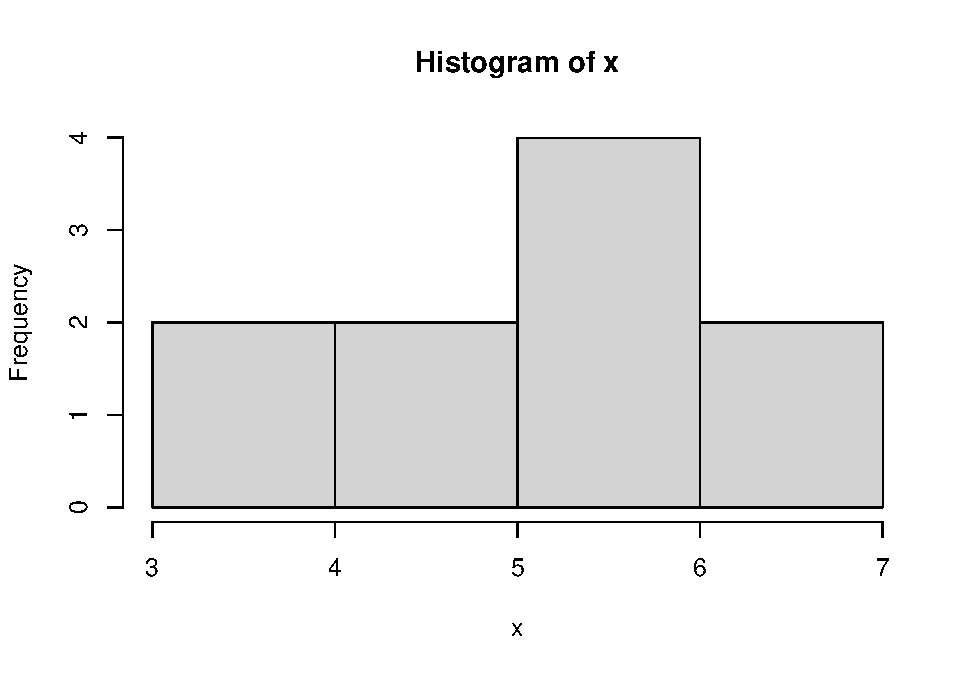
\includegraphics{Data-Science-Untuk-Pemula_files/figure-latex/unnamed-chunk-9-1.pdf}

R menyimpan setiap objek yang anda buat dalam RAM. Semua koleksi dari semua objek tersebut adalah ruang kerja yang dapat anda periksa dengan:

\begin{Shaded}
\begin{Highlighting}[]
\KeywordTok{ls}\NormalTok{ () 			                                    }\CommentTok{# Koleksi semua objek tersebut}
\KeywordTok{ls}\NormalTok{ (}\DataTypeTok{pattern =} \StringTok{'x'}\NormalTok{) 	                            }\CommentTok{# menggunakan ls dengan pola teks}
\KeywordTok{rm}\NormalTok{ (x) 			                                    }\CommentTok{# Menghapus variabel}
\KeywordTok{ls}\NormalTok{ () 		                                  	  }\CommentTok{# Memverifikasi}
\end{Highlighting}
\end{Shaded}

Anda mungkin berpikir bahwa jika suatu objek dihapus maka memorinya akan dilepaskan. Ini hampir benar, tergantung pada mekanisme negosiasi antara R dan sistem operasi.

\hypertarget{nilai-yang-hilang}{%
\section{Nilai yang Hilang}\label{nilai-yang-hilang}}

Tidak seperti pemrograman yang biasa, ketika bekerja dengan data di kehidupan nyata, anda mungkin mempunyai nilai yang hilang: pengukuran yang tidak direkam/disimpan/dll. R memiliki mekanisme yang agak canggih untuk menangani nilai-nilai yang hilang. Ini membedakan antara jenis atau tipe berikut:

\begin{itemize}
\tightlist
\item
  \texttt{NA}: Entri yang tidak tersedia (nilai \texttt{NA} juga memiliki kelas, jadi ada bilangan bulat \texttt{NA}, karakter NA, dll.)
\item
  \texttt{NaN}: Bukan angka (Nilai NaN juga \texttt{NA} tetapi sebaliknya tidak benar)
\end{itemize}

R mencoba mempertahankan analis dan mengembalikan kesalahan atau \texttt{NA} ketika keberadaan nilai yang hilang membuat perhitungan tidak valid:

\begin{Shaded}
\begin{Highlighting}[]
\NormalTok{missing.example <-}\StringTok{ }\KeywordTok{c}\NormalTok{(}\DecValTok{10}\NormalTok{,}\DecValTok{11}\NormalTok{,}\DecValTok{12}\NormalTok{,}\OtherTok{NA}\NormalTok{)                }\CommentTok{# Membuat vector dengan bilai yang hilang}
\KeywordTok{is.na}\NormalTok{(missing.example)                           }\CommentTok{# Memeriksa nilai yang hilang}
\KeywordTok{which}\NormalTok{(}\KeywordTok{is.na}\NormalTok{(missing.example))                    }\CommentTok{# Mengidentifikasi `NA` (hanya vector)}
\KeywordTok{mean}\NormalTok{(missing.example)                            }\CommentTok{# Menghitung rata-rata dengan nilai yang hilang}
\end{Highlighting}
\end{Shaded}

Sebagian besar fungsi biasanya memiliki mekanisme internal untuk menghadapi hal ini. Dalam fungsi rata-rata, ada argumen na.rm yang memberi tahu R cara menghapus \texttt{NA}.

\begin{Shaded}
\begin{Highlighting}[]
\KeywordTok{mean}\NormalTok{(missing.example, }\DataTypeTok{na.rm =} \OtherTok{TRUE}\NormalTok{)               }\CommentTok{# Rata-rata tanpa nilai yang hilang}
\end{Highlighting}
\end{Shaded}

Temukan nilai yang hilang di kolom data frame

\begin{Shaded}
\begin{Highlighting}[]
\NormalTok{df <-}\StringTok{ }\KeywordTok{data.frame}\NormalTok{( }\DataTypeTok{x1 =} \KeywordTok{c}\NormalTok{(}\OtherTok{NA}\NormalTok{, }\DecValTok{7}\NormalTok{, }\DecValTok{8}\NormalTok{, }\DecValTok{9}\NormalTok{, }\DecValTok{3}\NormalTok{),         }\CommentTok{# Variabel numerik dengan satu nilai hilang}
                  \DataTypeTok{x2 =} \KeywordTok{c}\NormalTok{(}\DecValTok{4}\NormalTok{, }\DecValTok{1}\NormalTok{, }\OtherTok{NA}\NormalTok{, }\OtherTok{NA}\NormalTok{, }\DecValTok{4}\NormalTok{),        }\CommentTok{# Variabel numerik dengan dua nilai hilang}
                  \DataTypeTok{x3 =} \KeywordTok{c}\NormalTok{(}\DecValTok{1}\NormalTok{, }\DecValTok{4}\NormalTok{, }\DecValTok{2}\NormalTok{, }\DecValTok{9}\NormalTok{, }\DecValTok{6}\NormalTok{),          }\CommentTok{# Variabel numerik tanpa nilai hilang}
                  \DataTypeTok{x4 =} \KeywordTok{c}\NormalTok{(}\StringTok{"Hello"}\NormalTok{, }\StringTok{"I am Bakti"}\NormalTok{, }
                         \OtherTok{NA}\NormalTok{, }\StringTok{"I love R"}\NormalTok{,}\OtherTok{NA}\NormalTok{))      }\CommentTok{# Variabel factor dengan}
\KeywordTok{is.na}\NormalTok{(df)                                         }\CommentTok{# Cara klasik untuk memeriksa `NA`}
\KeywordTok{sum}\NormalTok{(}\KeywordTok{is.na}\NormalTok{(df))                                    }\CommentTok{# Menghitung `NA`}
\KeywordTok{apply}\NormalTok{(}\KeywordTok{is.na}\NormalTok{(df),}\DecValTok{2}\NormalTok{, which)                         }\CommentTok{# Mengindeks `NA` (hanya df)}
\KeywordTok{which}\NormalTok{(}\KeywordTok{complete.cases}\NormalTok{(df))                         }\CommentTok{# Mengidentifikasi nilai yang diamati}
\end{Highlighting}
\end{Shaded}

Mekanisme yang lebih umum adalah menghapus ini secara manual:

\begin{Shaded}
\begin{Highlighting}[]
\NormalTok{clean.example <-}\StringTok{ }\KeywordTok{na.omit}\NormalTok{(missing.example)         }\CommentTok{# Menghapus vector `NA`}
\NormalTok{clean.df <-}\StringTok{ }\KeywordTok{na.omit}\NormalTok{(df)                           }\CommentTok{# Menghapus data frame `NA`}
\end{Highlighting}
\end{Shaded}

\hypertarget{piping}{%
\section{Piping}\label{piping}}

Karena R berasal mewarisi banyak sumber, juga mengadopsi OS seperti Unix dan Linux. \texttt{Piping} adalah ide yang diambil dari Linux shell yang memungkinkan untuk menggunakan output dari satu ekspresi sebagai input ke yang lain. Dengan demikian, Piping membuat kode lebih mudah dibaca dan ditulis.

\begin{Shaded}
\begin{Highlighting}[]
\CommentTok{# Prasyarat:}
\KeywordTok{library}\NormalTok{(magrittr)                                  }\CommentTok{# Memuat fungsi piping}
\CommentTok{# help(package = "magrittr")                       # Memuat informasi `magrittr`}
\NormalTok{x <-}\StringTok{ }\KeywordTok{rbinom}\NormalTok{(}\DataTypeTok{n=}\DecValTok{1000}\NormalTok{, }\DataTypeTok{size=}\DecValTok{10}\NormalTok{, }\DataTypeTok{prob=}\FloatTok{0.5}\NormalTok{)           	 }\CommentTok{# Menghasilkan beberapa sampel data}
\CommentTok{# Contoh:}
\NormalTok{x }\OperatorTok\StringTok{ }\KeywordTok{var}\NormalTok{()                                        }\CommentTok{# Bukan `var(x)`}
\NormalTok{x }\OperatorTok\StringTok{ }\KeywordTok{hist}\NormalTok{()                                     	 }\CommentTok{# Sebagai ganti `hist(x)`}
\end{Highlighting}
\end{Shaded}

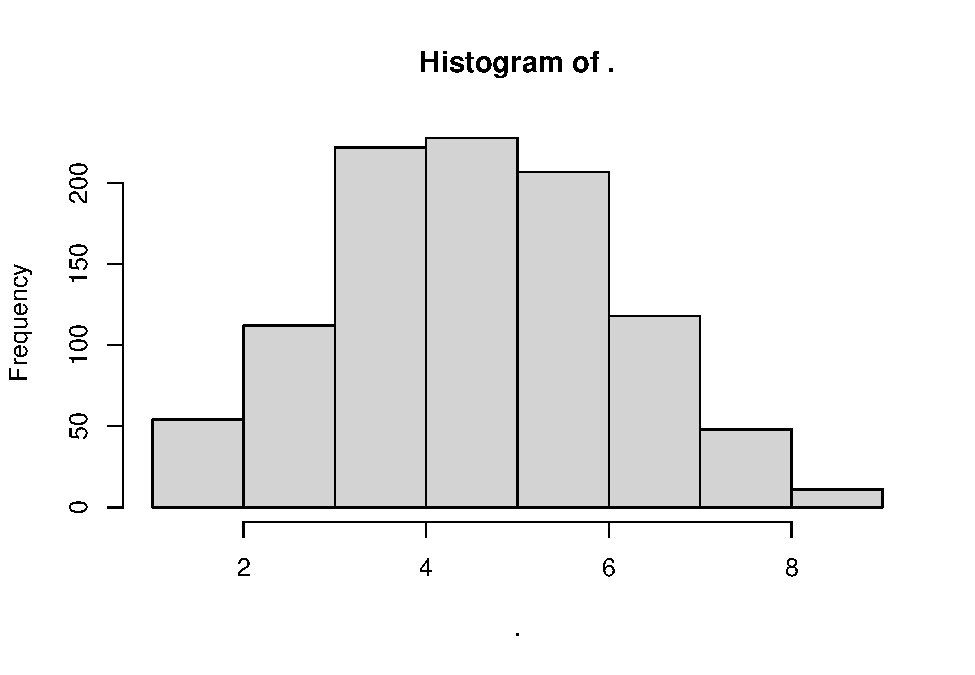
\includegraphics{Data-Science-Untuk-Pemula_files/figure-latex/unnamed-chunk-15-1.pdf}

\begin{Shaded}
\begin{Highlighting}[]
\NormalTok{x }\OperatorTok\StringTok{ }\KeywordTok{mean}\NormalTok{() }\OperatorTok\StringTok{ }\KeywordTok{round}\NormalTok{(}\DecValTok{2}\NormalTok{) }\OperatorTok\StringTok{ }\KeywordTok{add}\NormalTok{(}\DecValTok{10}\NormalTok{)              }\CommentTok{# Sebagai ganti beberapa fungsi}
\end{Highlighting}
\end{Shaded}

Contoh berikutnya menunjukkan manfaat dari piping. Dua potongan kode selanjutnya melakukan hal yang sama. Coba uraikan dalam pikiran Anda:

\begin{Shaded}
\begin{Highlighting}[]
\CommentTok{# Gaya fungsional Onion style}
\NormalTok{car_data <-}\StringTok{ }
\KeywordTok{transform}\NormalTok{(}\KeywordTok{aggregate}\NormalTok{(. }\OperatorTok{~}\StringTok{ }\NormalTok{cyl, }
                    \DataTypeTok{data =} \KeywordTok{subset}\NormalTok{(mtcars, hp }\OperatorTok{>}\StringTok{ }\DecValTok{100}\NormalTok{), }
                    \DataTypeTok{FUN =} \ControlFlowTok{function}\NormalTok{(x) }\KeywordTok{round}\NormalTok{(}\KeywordTok{mean}\NormalTok{(x, }\DecValTok{2}\NormalTok{))), }
                    \DataTypeTok{kpl =}\NormalTok{ mpg}\OperatorTok{*}\FloatTok{0.4251}\NormalTok{)}
\end{Highlighting}
\end{Shaded}

\begin{Shaded}
\begin{Highlighting}[]
\CommentTok{# Piping (magrittr) style}
\NormalTok{car_data <-}\StringTok{ }\NormalTok{mtcars }\OperatorTok
\StringTok{  }\KeywordTok{subset}\NormalTok{(hp }\OperatorTok{>}\StringTok{ }\DecValTok{100}\NormalTok{) }\OperatorTok
\StringTok{  }\KeywordTok{aggregate}\NormalTok{(. }\OperatorTok{~}\StringTok{ }\NormalTok{cyl, }\DataTypeTok{data =}\NormalTok{ ., }\DataTypeTok{FUN =}\NormalTok{ . }\OperatorTok\StringTok{ }\NormalTok{mean }\OperatorTok\StringTok{ }\KeywordTok{round}\NormalTok{(}\DecValTok{2}\NormalTok{)) }\OperatorTok
\StringTok{  }\KeywordTok{transform}\NormalTok{(}\DataTypeTok{kpl =}\NormalTok{ mpg }\OperatorTok\StringTok{ }\KeywordTok{multiply_by}\NormalTok{(}\FloatTok{0.4251}\NormalTok{)) }\OperatorTok
\StringTok{  }\NormalTok{print}
\end{Highlighting}
\end{Shaded}

Tip: RStudio memiliki jalan pintas melalui keyboard untuk \texttt{\%\textgreater{}\%} operator. Coba \texttt{Ctrl+Shift+m}.

\hypertarget{membuat-vektor}{%
\section{Membuat Vektor}\label{membuat-vektor}}

Elemen paling dasar dalam R adalah vektor. Kita sekarang akan melihat cara membuat vector dan mengakses elemen-elemen (yaitu, subset). Berikut adalah tiga cara untuk membuat vektor yang sama:

\begin{Shaded}
\begin{Highlighting}[]
\KeywordTok{c}\NormalTok{(}\DecValTok{10}\NormalTok{,}\DecValTok{11}\NormalTok{,}\DecValTok{12}\NormalTok{,}\DecValTok{13}\NormalTok{,}\DecValTok{14}\NormalTok{,}\DecValTok{15}\NormalTok{,}\DecValTok{16}\NormalTok{,}\DecValTok{17}\NormalTok{,}\DecValTok{18}\NormalTok{,}\DecValTok{19}\NormalTok{,}\DecValTok{20}\NormalTok{,}\DecValTok{21}\NormalTok{) 		  }\CommentTok{# Membuat vektor secara manual}
\DecValTok{10}\OperatorTok{:}\DecValTok{21}                                  			\CommentTok{# Menggunakan operator `:`}
\KeywordTok{seq}\NormalTok{(}\DataTypeTok{from=}\DecValTok{10}\NormalTok{, }\DataTypeTok{to=}\DecValTok{21}\NormalTok{, }\DataTypeTok{by=}\DecValTok{1}\NormalTok{)              		  }\CommentTok{# fungsi `seq()` dengan "by"}
\KeywordTok{seq}\NormalTok{(}\DataTypeTok{from=}\DecValTok{10}\NormalTok{, }\DataTypeTok{to=}\DecValTok{21}\NormalTok{, }\DataTypeTok{len=}\DecValTok{12}\NormalTok{)          		    }\CommentTok{# fungsi `seq()` dengan "len"}
\NormalTok{x <-}\StringTok{ }\DecValTok{10}\OperatorTok{:}\DecValTok{21}                             			\CommentTok{# Mari kita tetapkan ke objek bernama "x"}
\NormalTok{x}\OperatorTok{+}\DecValTok{2}                                    			\CommentTok{# Operasi biasanya bekerja berdasarkan elemen}
\NormalTok{x}\OperatorTok{*}\DecValTok{2}                                    			\CommentTok{# Tambahkan 2 untuk setiap elemen `x`}
\NormalTok{x}\OperatorTok{^}\DecValTok{2}                                    			\CommentTok{# Pangkat 2 untuk setiap elemen `x` }
\KeywordTok{sqrt}\NormalTok{(x)                                			}\CommentTok{# Akar kuadrat untuk setiap elemen ‘x’}
\KeywordTok{log}\NormalTok{(x)                                			}\CommentTok{# Logaritma untuk setiap elemen 'x’ }
\NormalTok{x <-}\StringTok{ }\KeywordTok{c}\NormalTok{(}\FloatTok{0.5}\NormalTok{, }\FloatTok{0.6}\NormalTok{)                       			}\CommentTok{# Numerik}
\NormalTok{x <-}\StringTok{ }\KeywordTok{c}\NormalTok{(}\OtherTok{TRUE}\NormalTok{, }\OtherTok{FALSE}\NormalTok{)                    			}\CommentTok{# Logis}
\NormalTok{x <-}\StringTok{ }\KeywordTok{c}\NormalTok{(T, F)                        				}\CommentTok{# Logis}
\NormalTok{x <-}\StringTok{ }\KeywordTok{c}\NormalTok{(}\StringTok{"a"}\NormalTok{, }\StringTok{"b"}\NormalTok{, }\StringTok{"c"}\NormalTok{)                  			}\CommentTok{# Karakter}
\NormalTok{x <-}\StringTok{ }\DecValTok{9}\OperatorTok{:}\DecValTok{29}                              			\CommentTok{# Integer}
\NormalTok{x <-}\StringTok{ }\KeywordTok{c}\NormalTok{(}\DecValTok{1}\OperatorTok{+}\NormalTok{0i, }\DecValTok{2}\OperatorTok{+}\NormalTok{4i)                     			}\CommentTok{# Complex}
\NormalTok{x <-}\StringTok{ }\KeywordTok{vector}\NormalTok{(}\StringTok{"numeric"}\NormalTok{, }\DataTypeTok{length =} \DecValTok{10}\NormalTok{)    		  }\CommentTok{# fungsi `vector ()` untuk menginisialisasi vektor.}
\NormalTok{y <-}\StringTok{ }\KeywordTok{c}\NormalTok{(}\FloatTok{1.7}\NormalTok{, }\StringTok{"a"}\NormalTok{)                      			}\CommentTok{# Karakter}
\NormalTok{y <-}\StringTok{ }\KeywordTok{c}\NormalTok{(}\OtherTok{TRUE}\NormalTok{, }\DecValTok{2}\NormalTok{)                     			  }\CommentTok{# Numerik}
\NormalTok{y <-}\StringTok{ }\KeywordTok{c}\NormalTok{(}\StringTok{"a"}\NormalTok{, }\OtherTok{TRUE}\NormalTok{)                      			}\CommentTok{# Numerik}
\KeywordTok{typeof}\NormalTok{(y)                              			}\CommentTok{# Untuk memeriksa jenis `y`}
\KeywordTok{class}\NormalTok{(y)                               			}\CommentTok{# Untuk memeriksa jenis `y`}
\end{Highlighting}
\end{Shaded}

\textbf{Catatan:} Menurut dokumentasi R untuk \texttt{typeof()} dan \texttt{class()}, pernyataan tentang ``perbedaan utama/ main difference'' adalah tidak benar. class adalah atribut dari objek yang dapat ditetapkan terlepas dari mode penyimpanan internalnya, sedangkan \texttt{typeof()} menentukan tipe (R internal) atau mode penyimpanan dari objek apa pun. Satu menggambarkan karakteristik logis sedangkan yang lain adalah karakteristik fisik dari suatu objek.

\begin{Shaded}
\begin{Highlighting}[]
\NormalTok{x <-}\StringTok{ }\DecValTok{0}\OperatorTok{:}\DecValTok{10}                              	   \CommentTok{# Mari tetapkan ke objek bernama `x`}
\KeywordTok{class}\NormalTok{(x)                               	   }\CommentTok{# Periksa kelas `x`}
\KeywordTok{as.numeric}\NormalTok{(x)                       	     }\CommentTok{# Menetapkan `x` sebagai numerik}
\KeywordTok{as.logical}\NormalTok{(x)                          	   }\CommentTok{# Menetapkan `x` sebagai logis}
\KeywordTok{as.character}\NormalTok{(x)                        	   }\CommentTok{# Menetapkan `x` sebagai karakter}
\KeywordTok{as.numeric}\NormalTok{(}\KeywordTok{c}\NormalTok{(}\OtherTok{FALSE}\NormalTok{,}\OtherTok{TRUE}\NormalTok{,}\OtherTok{TRUE}\NormalTok{,}\OtherTok{FALSE}\NormalTok{))       }\CommentTok{# Menetapkan vektor logis sebagai angka }
\end{Highlighting}
\end{Shaded}

Terkadang, R tidak dapat menemukan cara untuk memaksa suatu objek dan ini dapat menghasilkan NA.

\begin{Shaded}
\begin{Highlighting}[]
\NormalTok{x <-}\StringTok{ }\KeywordTok{c}\NormalTok{(}\StringTok{"a"}\NormalTok{, }\StringTok{"b"}\NormalTok{, }\StringTok{"c"}\NormalTok{,}\StringTok{"1"}\NormalTok{)       	         }\CommentTok{# menetapkan nilai `x`}
\KeywordTok{as.numeric}\NormalTok{(x)                          	   }\CommentTok{# menetapkan `x` sebagai numerik}
\end{Highlighting}
\end{Shaded}

\begin{verbatim}
## Warning: NAs introduced by coercion
\end{verbatim}

\begin{Shaded}
\begin{Highlighting}[]
\KeywordTok{as.logical}\NormalTok{(x)                        	     }\CommentTok{# menetapkan `x` sebagai logis}
\KeywordTok{as.complex}\NormalTok{(x)                        	     }\CommentTok{# menetapkan `x` sebagai karakter}
\end{Highlighting}
\end{Shaded}

\begin{verbatim}
## Warning: NAs introduced by coercion
\end{verbatim}

\textbf{Catatan:} Saat paksaan tidak masuk akal terjadi, anda biasanya akan mendapat peringatan dari R.

Kita sudah melihat bahwa elemen dasar dari objek R adalah vektor. Vektor dapat ditetapkan dengan berbagai jenis berikut:

\begin{itemize}
\tightlist
\item
  Karakter (character): di mana setiap elemen adalah string, mis., urutan simbol alfanumerik.
\item
  numeric (numeric) : Dimana setiap elemen adalah bilangan real dalam format floating point presisi ganda (double precision floating point format).
\item
  integer: di mana setiap elemen adalah integer.
\item
  logis: di mana setiap elemen adalah TRUE, FALSE, atau NA3
\item
  complex: di mana setiap elemen adalah bilangan kompleks.
\end{itemize}

\hypertarget{matriks}{%
\section{Matriks}\label{matriks}}

Matriks adalah vektor dengan atribut dimensi. Atribut dimensi itu sendiri merupakan vektor integer dengan panjang 2 (jumlah baris, jumlah kolom)

\begin{Shaded}
\begin{Highlighting}[]
\NormalTok{m <-}\StringTok{ }\KeywordTok{matrix}\NormalTok{(}\DataTypeTok{nrow =} \DecValTok{2}\NormalTok{, }\DataTypeTok{ncol =} \DecValTok{3}\NormalTok{)          }\CommentTok{# Membuat matriks `NA` sebanyak 2x3}
\NormalTok{m                                        }\CommentTok{# Mencetak hasilnya}
\KeywordTok{dim}\NormalTok{(m)                                   }\CommentTok{# Memeriksa dimensi}
\KeywordTok{attributes}\NormalTok{(m)                            }\CommentTok{# Memeriksa dimensi}
\end{Highlighting}
\end{Shaded}

Matriks dibuat berdasarkan kolom, sehingga entri dapat dianggap dimulai dari sudut ``kiri atas'' dan mengalir di kolom.

\begin{Shaded}
\begin{Highlighting}[]
\NormalTok{m <-}\StringTok{ }\KeywordTok{matrix}\NormalTok{ (}\DecValTok{1}\OperatorTok{:}\StringTok{ }\DecValTok{6}\NormalTok{, }\DataTypeTok{nrow =} \DecValTok{2}\NormalTok{, }\DataTypeTok{ncol =} \DecValTok{3}\NormalTok{)   }\CommentTok{# Membuat sebuah matriks dengan 2x3}
\end{Highlighting}
\end{Shaded}

Matriks juga dapat dibuat langsung dari vektor dengan menambahkan atribut dimensi.

\begin{Shaded}
\begin{Highlighting}[]
\NormalTok{m <-}\StringTok{ }\DecValTok{1}\OperatorTok{:}\DecValTok{10}                                \CommentTok{# Membuat vektor `m`}
\KeywordTok{dim}\NormalTok{(m) <-}\StringTok{ }\KeywordTok{c}\NormalTok{(}\DecValTok{2}\NormalTok{, }\DecValTok{5}\NormalTok{)                        }\CommentTok{# Menetapkan vektor `m` sebagai matriks sebesar 2x5}
\NormalTok{m                                        }\CommentTok{# Mencetak hasilnya}
\end{Highlighting}
\end{Shaded}

Matriks dapat dibuat dengan pengikatan kolom atau pengikatan baris dengan fungsi \texttt{cbind()} dan \texttt{rbind()}.

\begin{Shaded}
\begin{Highlighting}[]
\NormalTok{x <-}\StringTok{ }\DecValTok{1}\OperatorTok{:}\DecValTok{3}                                 \CommentTok{# Membuat vektor `x`}
\NormalTok{y <-}\StringTok{ }\DecValTok{10}\OperatorTok{:}\DecValTok{12}                               \CommentTok{# Membuat vektor `y`}
\KeywordTok{cbind}\NormalTok{(x, y)                              }\CommentTok{# Menggabungkan vektor `x` dan` y` dengan kolom}
\KeywordTok{rbind}\NormalTok{(x, y)                              }\CommentTok{# Menggabungkan vektor `x` dan` y` dengan baris}
\end{Highlighting}
\end{Shaded}

\hypertarget{list}{%
\section{List}\label{list}}

Daftar (List) adalah jenis vektor khusus yang dapat berisi elemen dari kelas yang berbeda. List merupakan tipe data yang sangat penting dalam R dan anda harus mengenalnya dengan baik. List, dalam kombinasi dengan berbagai fungsi ``terapkan (apply)'' yang akan dibahas nanti, membuat kombinasi yang kuat. List dapat dibuat secara eksplisit menggunakan fungsi \texttt{list()}, yang mengambil sejumlah argumen arbitrer.

Secara umum anda dapat menggunakan dua operasi pengindeksan yang berbeda pada List:

\begin{itemize}
\tightlist
\item
  Kurung tunggal untuk mengembalikan daftar elemen yang dipilih \texttt{({[}{]})}
\item
  Kurung ganda untuk mengembalikan elemen tunggal \texttt{({[}{[}{]}{]})}
\end{itemize}

\begin{Shaded}
\begin{Highlighting}[]
\NormalTok{x <-}\StringTok{ }\KeywordTok{list}\NormalTok{(}\DecValTok{1}\OperatorTok{:}\DecValTok{5}\NormalTok{,}\KeywordTok{c}\NormalTok{(}\StringTok{"a"}\NormalTok{,}\StringTok{"b"}\NormalTok{,}\StringTok{"c"}\NormalTok{),}\OtherTok{TRUE}\NormalTok{,}\DecValTok{7}\NormalTok{,}\DecValTok{5}\NormalTok{)  }\CommentTok{# Membuat daftar (list) vektor `x`}
\NormalTok{x[}\DecValTok{1}\NormalTok{]                                    }\CommentTok{# Kurung tunggal}
\NormalTok{x[[}\DecValTok{1}\NormalTok{]]                                  }\CommentTok{# Kurung ganda}
\KeywordTok{typeof}\NormalTok{(x[}\DecValTok{2}\NormalTok{])                            }\CommentTok{# Memeriksa jenis objek menggunakan []}
\KeywordTok{typeof}\NormalTok{(x[[}\DecValTok{2}\NormalTok{]])                          }\CommentTok{# Memeriksa jenis objek menggunakan [[]]}
\NormalTok{x[}\KeywordTok{c}\NormalTok{(}\DecValTok{1}\NormalTok{,}\DecValTok{2}\NormalTok{)]                               }\CommentTok{# list vektor pertama dan kedua}
\end{Highlighting}
\end{Shaded}

Kami juga dapat membuat daftar (list) dengan mengganti objek kosong yang ada seperti yang anda lihat dalam kode berikut:

\begin{Shaded}
\begin{Highlighting}[]
\NormalTok{x <-}\StringTok{ }\KeywordTok{vector}\NormalTok{(}\StringTok{"list"}\NormalTok{, }\DataTypeTok{length =} \DecValTok{3}\NormalTok{)         }\CommentTok{# Membuat daftar (list) kosong (sesuai kebutuhan)}
\NormalTok{name <-}\StringTok{ }\KeywordTok{c}\NormalTok{(}\StringTok{"a"}\NormalTok{,}\StringTok{"b"}\NormalTok{,}\StringTok{"c"}\NormalTok{,}\StringTok{"d"}\NormalTok{)              }\CommentTok{# Membuat objek sebagai variabel `name`}
\NormalTok{age  <-}\StringTok{ }\KeywordTok{c}\NormalTok{(}\DecValTok{18}\NormalTok{, }\DecValTok{19}\NormalTok{, }\DecValTok{20}\NormalTok{, }\DecValTok{21}\NormalTok{)               }\CommentTok{# Membuat objek sebagai variabel `age`}
\NormalTok{gender<-}\StringTok{ }\KeywordTok{c}\NormalTok{(}\DecValTok{1}\NormalTok{, }\DecValTok{0}\NormalTok{, }\DecValTok{0}\NormalTok{, }\DecValTok{1}\NormalTok{)                  }\CommentTok{# Membuat objek sebagai variabel `gender`}
\NormalTok{x[[}\DecValTok{1}\NormalTok{]] <-}\StringTok{ }\NormalTok{name                          }\CommentTok{# Tambah / ganti objek ke daftar `x`}
\NormalTok{x[[}\DecValTok{2}\NormalTok{]] <-}\StringTok{ }\NormalTok{age                           }\CommentTok{# Tambah / ganti objek ke daftar `x`}
\NormalTok{x[[}\DecValTok{3}\NormalTok{]] <-}\StringTok{ }\NormalTok{gender                        }\CommentTok{# Tambah / ganti objek ke daftar `x`}
\NormalTok{x                                       }\CommentTok{# Cetak hasil akhir}
\end{Highlighting}
\end{Shaded}

\hypertarget{factor}{%
\section{Factor}\label{factor}}

Faktor-faktor digunakan untuk mewakili data kategorikal dan dapat menjadi tidak teratur atau teratur. Orang dapat menganggap faktor sebagai vektor integer di mana setiap integer memiliki label. Faktor-faktor menjadi penting dalam pemodelan statistik dan diperlakukan secara khusus oleh fungsi pemodelan seperti \texttt{lm()} dan \texttt{glm()}.
Menggunakan faktor dengan label lebih baik daripada menggunakan bilangan bulat karena faktor menggambarkan diri sendiri. Memiliki variabel yang memiliki nilai ``Pria'' dan ``Wanita'' lebih baik daripada variabel yang memiliki nilai 1 dan 2. Objek objek dapat dibuat dengan fungsi \texttt{faktor()}.

\begin{Shaded}
\begin{Highlighting}[]
\NormalTok{x <-}\StringTok{ }\KeywordTok{factor}\NormalTok{(}\KeywordTok{c}\NormalTok{(}\StringTok{"yes"}\NormalTok{,}\StringTok{"no"}\NormalTok{,}\StringTok{"yes"}\NormalTok{,}\StringTok{"no"}\NormalTok{))  }\CommentTok{# Membuat objek faktor}
\NormalTok{x                                      }\CommentTok{# Cetak hasilnya}
\KeywordTok{table}\NormalTok{(x)                               }\CommentTok{# Tabel dari `x`}
\KeywordTok{unclass}\NormalTok{(x)                             }\CommentTok{# Melihat representasi faktor yang mendasarinya}
\KeywordTok{attr}\NormalTok{(x,}\StringTok{"levels"}\NormalTok{)                       }\CommentTok{# Melihat representasi faktor yang mendasarinya}
\end{Highlighting}
\end{Shaded}

\hypertarget{data-frame}{%
\section{Data Frame}\label{data-frame}}

Kerangka data (data frame) adalah tabel atau struktur mirip array dua dimensi di mana setiap kolom berisi nilai satu variabel dan setiap baris berisi satu set nilai dari setiap kolom.
Berikut ini adalah karakteristik data frame.

\begin{itemize}
\tightlist
\item
  Nama kolom tidak boleh kosong;
\item
  Nama baris harus unik;
\item
  Data yang disimpan dalam data frame bisa dari numerik, faktor atau tipe karakter;
\item
  Setiap kolom harus berisi jumlah item data yang sama.
\end{itemize}

\begin{Shaded}
\begin{Highlighting}[]
\CommentTok{# Buat data frame pertama.}
\NormalTok{df1 <-}\StringTok{ }\KeywordTok{data.frame}\NormalTok{(}\DataTypeTok{id =} \KeywordTok{c}\NormalTok{ (}\DecValTok{1}\OperatorTok{:}\DecValTok{5}\NormalTok{), }
                \DataTypeTok{name =} \KeywordTok{c}\NormalTok{(}\StringTok{"Julian"}\NormalTok{,}\StringTok{"Vanessa"}\NormalTok{,}\StringTok{"Jeffry"}\NormalTok{,}\StringTok{"Angel"}\NormalTok{,}\StringTok{"Nikki"}\NormalTok{),}
              \DataTypeTok{salary =} \KeywordTok{c}\NormalTok{(}\FloatTok{623.3}\NormalTok{,}\FloatTok{515.2}\NormalTok{,}\FloatTok{611.0}\NormalTok{,}\FloatTok{729.0}\NormalTok{,}\FloatTok{843.25}\NormalTok{), }
          \DataTypeTok{start_date =} \KeywordTok{as.Date}\NormalTok{(}\KeywordTok{c}\NormalTok{(}\StringTok{"2022-01-01"}\NormalTok{, }\StringTok{"2022-09-23"}\NormalTok{, }\StringTok{"2022-11-15"}\NormalTok{,                                               }\StringTok{"2022-05-11"}\NormalTok{, }\StringTok{"2022-03-27"}\NormalTok{)),}
                \DataTypeTok{dept =} \KeywordTok{c}\NormalTok{(}\StringTok{"DS"}\NormalTok{,}\StringTok{"DS"}\NormalTok{,}\StringTok{"BA"}\NormalTok{,}\StringTok{"DA"}\NormalTok{,}\StringTok{"DS"}\NormalTok{), }\DataTypeTok{stringsAsFactors =}\NormalTok{ F)}
\NormalTok{df1}
\end{Highlighting}
\end{Shaded}

\begin{Shaded}
\begin{Highlighting}[]
\CommentTok{# Buat data frame kedua.}
\NormalTok{df2 <-}\KeywordTok{data.frame}\NormalTok{(}\DataTypeTok{id =} \KeywordTok{c}\NormalTok{ (}\DecValTok{6}\OperatorTok{:}\DecValTok{10}\NormalTok{), }
               \DataTypeTok{name =} \KeywordTok{c}\NormalTok{(}\StringTok{"Ardifo"}\NormalTok{,}\StringTok{"Irene"}\NormalTok{,}\StringTok{"Kefas"}\NormalTok{,}\StringTok{"Sherly"}\NormalTok{,}\StringTok{"Bakti"}\NormalTok{),}
             \DataTypeTok{salary =} \KeywordTok{c}\NormalTok{(}\FloatTok{578.0}\NormalTok{,}\FloatTok{722.5}\NormalTok{,}\FloatTok{632.8}\NormalTok{,}\FloatTok{632.8}\NormalTok{,}\OtherTok{NA}\NormalTok{), }
         \DataTypeTok{start_date =} \KeywordTok{as.Date}\NormalTok{(}\KeywordTok{c}\NormalTok{(}\StringTok{"2022-05-21"}\NormalTok{,}\StringTok{"2022-07-30"}\NormalTok{,}\StringTok{"2022-06-17"}\NormalTok{,}
                                \StringTok{"2022-07-30"}\NormalTok{,}\StringTok{"2018-09-03"}\NormalTok{)),}
               \DataTypeTok{dept =} \KeywordTok{c}\NormalTok{(}\StringTok{"Actuaries"}\NormalTok{,}\StringTok{"Actuaries"}\NormalTok{,}\StringTok{"CA"}\NormalTok{,}\StringTok{"DE"}\NormalTok{,}\StringTok{"Lecturer"}\NormalTok{),}\DataTypeTok{stringsAsFactors =}\NormalTok{ F)}
\NormalTok{df2}
\end{Highlighting}
\end{Shaded}

\begin{Shaded}
\begin{Highlighting}[]
\NormalTok{df3 <-}\StringTok{ }\KeywordTok{rbind}\NormalTok{(df1,df2)                  }\CommentTok{# Gabungkan dua frame data}
\KeywordTok{print}\NormalTok{(df3)                             }\CommentTok{# Cetak hasilnya `df3`}
\KeywordTok{head}\NormalTok{(df3)                              }\CommentTok{# Cetak enam baris pertama}
\KeywordTok{head}\NormalTok{(df3,}\DecValTok{6}\NormalTok{)                            }\CommentTok{# Cetak enam baris pertama}
\CommentTok{#View(df3)                             # Menggunakan RStudio seperti penampil Excel}
\KeywordTok{class}\NormalTok{(df3)                             }\CommentTok{# objeknya bertipe data.frame}
\KeywordTok{str}\NormalTok{(df3)                               }\CommentTok{# Dapatkan struktur data frame}
\KeywordTok{dim}\NormalTok{(df3)                               }\CommentTok{# Periksa dimensi data}
\end{Highlighting}
\end{Shaded}

Data frame biasanya dibuat dengan membaca dalam dataset menggunakan \texttt{read.table()} atau \texttt{read.csv\ ()}. Namun, data frame juga dapat dibuat secara eksplisit dengan fungsi \texttt{data.frame()} atau mereka dapat dipaksakan dari jenis objek lain seperti list.

\hypertarget{names}{%
\section{Names}\label{names}}

Objek R dapat memiliki nama, yang sangat berguna untuk menulis kode yang dapat dibaca dan menggambarkan objek sendiri. Berikut adalah contoh pemberian nama ke vektor integer.

\begin{Shaded}
\begin{Highlighting}[]
\NormalTok{data<-df1                              }\CommentTok{# Panggil `df1` seperti yang kita gunakan di bagian sebelumnya}
\KeywordTok{names}\NormalTok{(data)                            }\CommentTok{# Periksa nama variabel data}
\end{Highlighting}
\end{Shaded}

\begin{verbatim}
## [1] "id"         "name"       "salary"     "start_date" "dept"
\end{verbatim}

\begin{Shaded}
\begin{Highlighting}[]
\KeywordTok{names}\NormalTok{(data)<-}\KeywordTok{c}\NormalTok{(}\StringTok{"no"}\NormalTok{, }\StringTok{"nama"}\NormalTok{, }\StringTok{"gaji"}\NormalTok{,}
             \StringTok{"mulai_bekerja"}\NormalTok{,}\StringTok{"divisi"}\NormalTok{) }\CommentTok{# Mengubah nama nama variabel menjadi Indonesia}
\NormalTok{data                                   }\CommentTok{# Cetak hasilnya}
\end{Highlighting}
\end{Shaded}

\begin{verbatim}
##   no    nama   gaji mulai_bekerja divisi
## 1  1  Julian 623.30    2022-01-01     DS
## 2  2 Vanessa 515.20    2022-09-23     DS
## 3  3  Jeffry 611.00    2022-11-15     BA
## 4  4   Angel 729.00    2022-05-11     DA
## 5  5   Nikki 843.25    2022-03-27     DS
\end{verbatim}

Matriks dapat memiliki nama kolom dan baris.

\begin{Shaded}
\begin{Highlighting}[]
\NormalTok{m <-}\StringTok{ }\KeywordTok{matrix}\NormalTok{(}\DecValTok{1}\OperatorTok{:}\DecValTok{4}\NormalTok{, }\DataTypeTok{nrow =} \DecValTok{2}\NormalTok{, }\DataTypeTok{ncol =} \DecValTok{2}\NormalTok{)}
\KeywordTok{dimnames}\NormalTok{(m) <-}\StringTok{ }\KeywordTok{list}\NormalTok{(}\KeywordTok{c}\NormalTok{(}\StringTok{"a"}\NormalTok{, }\StringTok{"b"}\NormalTok{), }\KeywordTok{c}\NormalTok{(}\StringTok{"c"}\NormalTok{, }\StringTok{"d"}\NormalTok{)) }
\NormalTok{m}
\end{Highlighting}
\end{Shaded}

\begin{verbatim}
##   c d
## a 1 3
## b 2 4
\end{verbatim}

Nama kolom dan nama baris dapat diatur secara terpisah menggunakan fungsi \texttt{colnames()} dan \texttt{rownames()}.

\begin{Shaded}
\begin{Highlighting}[]
\KeywordTok{colnames}\NormalTok{(m) <-}\StringTok{ }\KeywordTok{c}\NormalTok{(}\StringTok{"h"}\NormalTok{, }\StringTok{"f"}\NormalTok{)}
\KeywordTok{rownames}\NormalTok{(m) <-}\StringTok{ }\KeywordTok{c}\NormalTok{(}\StringTok{"x"}\NormalTok{, }\StringTok{"z"}\NormalTok{)}
\NormalTok{m}
\end{Highlighting}
\end{Shaded}

\begin{verbatim}
##   h f
## x 1 3
## z 2 4
\end{verbatim}

Catatan: Dalam data frame, ada fungsi terpisah untuk mengatur nama baris, fungsi \texttt{row.names()}. Juga, data frane tidak memiliki nama kolom, mereka hanya memiliki nama (seperti list). Jadi untuk mengatur nama kolom dari data frame gunakan saja fungsi \texttt{names()}. Ya, saya tahu ini membingungkan. Berikut ringkasan singkatnya:

\begin{longtable}[]{@{}lll@{}}
\toprule
Objek T & etapkan nama kolom & Tetapkan nama baris\tabularnewline
\midrule
\endhead
data frame & names() & row.names()\tabularnewline
matrix & colnames() & rownames()\tabularnewline
\bottomrule
\end{longtable}

\hypertarget{pengeculian-ekstraksi}{%
\section{Pengeculian (Ekstraksi)}\label{pengeculian-ekstraksi}}

R menyediakan banyak cara untuk mengelompokkan dan mengekstrak elemen dari vektor dan objek lainnya. Dasar-dasarnya cukup sederhana, tetapi dengan tidak memperhatikan ``kepribadian'' dari setiap mekanisme ekstraksi dapat menyebabkan anda sakit kepala. Sebagai permulaan, ekstraksi dilakukan dengan operator \texttt{{[}{]}}. Operator dapat mengambil vektor dari banyak jenis.

\begin{Shaded}
\begin{Highlighting}[]
\CommentTok{#View(mtcars)                          # Lihat dataset `mtcars` (lingkungan R)}
\CommentTok{#?mtcars                               # Informasi detail tentang mtcars}
\KeywordTok{typeof}\NormalTok{(mtcars)                         }\CommentTok{# Periksa jenis data}
\KeywordTok{class}\NormalTok{(mtcars)                          }\CommentTok{# Periksa jenis data}
\NormalTok{mtcars[}\DecValTok{1}\NormalTok{,}\DecValTok{5}\NormalTok{]                            }\CommentTok{# Ekstrak elemen di baris 1 dan kolom 5.}
\NormalTok{mtcars[}\DecValTok{1}\OperatorTok{:}\DecValTok{5}\NormalTok{,]                           }\CommentTok{# Ekstrak enam baris pertama mtcars}
\NormalTok{mtcars[,}\DecValTok{1}\OperatorTok{:}\DecValTok{5}\NormalTok{]                           }\CommentTok{# Ekstrak enam kolom mtcars pertama}
\NormalTok{mtcars[,}\StringTok{'mpg'}\NormalTok{]                         }\CommentTok{# Ekstrak kolom khusus}
\NormalTok{mtcars}\OperatorTok{$}\NormalTok{mpg                             }\CommentTok{# Ekstrak kolom khusus}
\NormalTok{mtcars[}\StringTok{'Mazda RX4'}\NormalTok{,]                   }\CommentTok{# Ekstrak baris khusus}

\KeywordTok{subset}\NormalTok{(mtcars, }\DataTypeTok{select=}\NormalTok{mpg)             }\CommentTok{# Ekstrak / subset kolom spesifik}
\KeywordTok{subset}\NormalTok{(mtcars, }\DataTypeTok{select=}\DecValTok{1}\NormalTok{)               }\CommentTok{# Ekstrak / subset kolom spesifik}
\KeywordTok{subset}\NormalTok{(mtcars, }\DataTypeTok{select=} \KeywordTok{c}\NormalTok{(}\DecValTok{1}\NormalTok{,}\DecValTok{2}\NormalTok{))         }\CommentTok{# Ekstrak / subset kolom pertama & kedua}
\KeywordTok{subset}\NormalTok{(mtcars, }\DataTypeTok{select=} \KeywordTok{c}\NormalTok{(}\DecValTok{1}\OperatorTok{:}\DecValTok{5}\NormalTok{))         }\CommentTok{# Ekstrak / subset kolom spesifik}

\KeywordTok{min}\NormalTok{(mtcars}\OperatorTok{$}\NormalTok{mpg )                       }\CommentTok{# Temukan minimum gallon Miles/(US) }
\KeywordTok{max}\NormalTok{(mtcars}\OperatorTok{$}\NormalTok{mpg , }\DataTypeTok{na.rm =} \OtherTok{TRUE}\NormalTok{)         }\CommentTok{# Temukan maksimum gallon Miles/(US)}
\KeywordTok{mean}\NormalTok{(mtcars}\OperatorTok{$}\NormalTok{mpg , }\DataTypeTok{na.rm =} \OtherTok{TRUE}\NormalTok{)        }\CommentTok{# Temukan rata-rata gallon Miles/(US)}
\KeywordTok{var}\NormalTok{(mtcars}\OperatorTok{$}\NormalTok{mpg , }\DataTypeTok{na.rm =} \OtherTok{TRUE}\NormalTok{)         }\CommentTok{# Temukan varians gallon Miles/(US)}
\KeywordTok{sd}\NormalTok{(mtcars}\OperatorTok{$}\NormalTok{mpg , }\DataTypeTok{na.rm =} \OtherTok{TRUE}\NormalTok{)          }\CommentTok{# Temukan standar deviasi gallon Miles/(US)}
\end{Highlighting}
\end{Shaded}

Menambahkan variabel ke data.frame dapat dilakukan dengan menetapkan vektor baru. Kekuatan objek data.frame adalah bahwa data.frame menerima hampir semua jenis vektor, yaitu bilangan bulat, numerik, logis, faktor, dan karakter.

\begin{Shaded}
\begin{Highlighting}[]
\NormalTok{mtcars}\OperatorTok{$}\NormalTok{newvar1 <-}\StringTok{ }\NormalTok{mtcars}\OperatorTok{$}\NormalTok{mpg }\OperatorTok{-}\StringTok{ }\NormalTok{mtcars}\OperatorTok{$}\NormalTok{qsec}
\NormalTok{mtcars}\OperatorTok{$}\NormalTok{newvar2 <-}\StringTok{ }\NormalTok{mtcars}\OperatorTok{$}\NormalTok{newvar1 }\OperatorTok{>}\StringTok{ }\DecValTok{0}
\NormalTok{mtcars}\OperatorTok{$}\NormalTok{newvar3 <-}\StringTok{ }\KeywordTok{ifelse}\NormalTok{(mtcars}\OperatorTok{$}\NormalTok{newvar2, }\StringTok{"good"}\NormalTok{, }\StringTok{"bad"}\NormalTok{)}
\NormalTok{mtcars}\OperatorTok{$}\NormalTok{newvar4 <-}\StringTok{ }\KeywordTok{factor}\NormalTok{(mtcars}\OperatorTok{$}\NormalTok{newvar1}\OperatorTok{>}\DecValTok{10} \OperatorTok{&}\StringTok{ }\NormalTok{mtcars}\OperatorTok{$}\NormalTok{newvar3}\OperatorTok{==}\StringTok{"good"}\NormalTok{,}
                         \DataTypeTok{labels =} \KeywordTok{c}\NormalTok{(}\StringTok{"level1"}\NormalTok{,}\StringTok{"level2"}\NormalTok{))}
\end{Highlighting}
\end{Shaded}

\hypertarget{petunjuk-penting}{%
\section{Petunjuk Penting}\label{petunjuk-penting}}

Beberapa petunjuk bermanfaat untuk Rstudio (IDE) meliputi:

\begin{longtable}[]{@{}lcc@{}}
\toprule
Kata Kunci & Perintah & Detail\tabularnewline
\midrule
\endhead
Ctrl + Return (Enter) & untuk menjalankan baris dari editor & \textasciitilde{}\tabularnewline
Ctrl + Shift + \# & untuk fokus pada tab bantuan & kontradiktif\tabularnewline
Alt + Shift + k & untuk jalur pintas keyboard RStudio & \textasciitilde{}\tabularnewline
Ctrl + r & untuk menelusuri sejarah perintah & \textasciitilde{}\tabularnewline
Alt + Shift + j & untuk menavigasi antar bagian kode & \textasciitilde{}\tabularnewline
Ctrl + 1 & untuk melompat ke editor & tab untuk penyelesaian otomatis\tabularnewline
Ctrl + 2 & untuk melompat ke konsol & tab untuk penyelesaian otomatis\tabularnewline
Ctrl + 8 & untuk melompat ke environment list & tab untuk pelengkapan otomatis\tabularnewline
Alt + l & Collapse chunk & Code Folding\tabularnewline
Alt + Shift + l & Unfold chunk & Code Folding\tabularnewline
Alt + o & Collapse all & Code Folding\tabularnewline
Alt + Shift + o & Unfold all & Code Folding\tabularnewline
Alt + ``-'' & untuk operator penugasan \textless- & \textasciitilde{}\tabularnewline
Alt + Shift + c & kode komentar/tanda komentar dalam file & .R kontradiktif\tabularnewline
\bottomrule
\end{longtable}

Saat ini, saya sarankan anda untuk menggunakan RStudio di komputer (PC) anda, tetapi di sini saya sarankan beberapa IDE lain:

\begin{itemize}
\tightlist
\item
  Jupyter Lab: IDE yang sangat menjanjikan, awalnya dirancang untuk Python, yang juga mendukung R. Pada saat penulisan ini, tampaknya RStudio lebih nyaman untuk R, tetapi itu jelas merupakan IDE yang harus diikuti. Lihat ulasan Max Woolf.
\item
  Eclipse: Jika anda seorang programmer Java, anda mungkin akrab dengan Eclipse, yang memang memiliki R plugin: StatEt.
\item
  Emacs: Jika anda adalah penggemar Emacs, anda dapat menemukan R plugin: ESS.
\item
  Visual Studio juga mendukung R. Jika anda membutuhkan R untuk tujuan komersial, mungkin ada baiknya mencoba Microsoft's R, daripada R biasa. Lihat di sini untuk petunjuk pemasangan.
\end{itemize}

\hypertarget{Pemrograman-R}{%
\chapter{Pemrograman R}\label{Pemrograman-R}}

We describe our methods in this chapter.

\hypertarget{Interface-Data}{%
\chapter{Interface Data}\label{Interface-Data}}

\begin{center}\rule{0.5\linewidth}{0.5pt}\end{center}

Dengan R, kita dapat membaca data dari file yang tersimpan di luar Environment R. Kita juga dapat menulis data menjadi bentuk file yang akan disimpan dan diakses oleh sistem operasi. R dapat membaca dan menulis ke beberapa format file seperti \texttt{csv,\ excel,\ txt,\ rds,\ xml,\ json,\ dll}.

\hypertarget{direktori-kerja-working-directory}{%
\section{Direktori Kerja (Working Directory)}\label{direktori-kerja-working-directory}}

Sebelum kita mulai bekerja menggunakan data (data interface), pertama-tama pastikan working directory Anda berada di koneksi yang tepat. Anda dapat memeriksanya menggunakan fungsi \texttt{getwd()}. Anda juga dapat mengeset sebuah working directory baru menggunakan fungsi \texttt{setwd()}.

\begin{Shaded}
\begin{Highlighting}[]
\KeywordTok{print}\NormalTok{(}\KeywordTok{getwd}\NormalTok{())                                    }\CommentTok{# memperoleh dan mencetak working directory}
\end{Highlighting}
\end{Shaded}

\begin{verbatim}
## [1] "C:/Users/Bakti/Desktop/Website/Data-Science-Untuk-Pemula"
\end{verbatim}

\begin{Shaded}
\begin{Highlighting}[]
\KeywordTok{getwd}\NormalTok{()                                           }\CommentTok{# memperoleh dan mencetak working directory }
\end{Highlighting}
\end{Shaded}

\begin{verbatim}
## [1] "C:/Users/Bakti/Desktop/Website/Data-Science-Untuk-Pemula"
\end{verbatim}

\begin{Shaded}
\begin{Highlighting}[]
\CommentTok{#setwd("C:/Users/Bakti/Desktop/")                 # mengeset working directory Anda }
\CommentTok{#setwd("C:\textbackslash{}\textbackslash{}Users\textbackslash{}\textbackslash{}Bakti\textbackslash{}\textbackslash{}Desktop\textbackslash{}\textbackslash{}")             # atau dengan cara ini}
\end{Highlighting}
\end{Shaded}

\hypertarget{membacamenulis-csv}{%
\section{Membaca/Menulis CSV}\label{membacamenulis-csv}}

Ini adalah sebuah contoh sederhana dari fungsi \texttt{read.csv} untuk membaca sebuah file CSV yang tersedia di working directory Anda saat ini.

\begin{Shaded}
\begin{Highlighting}[]
\CommentTok{# csv <- read.csv(file.choose())                  # tampilan file csv tanpa `setwd`}
\NormalTok{csv1 <-}\StringTok{ }\KeywordTok{read.csv}\NormalTok{(}\StringTok{"Data/csv1.csv"}\NormalTok{,}\DataTypeTok{sep =} \StringTok{","}\NormalTok{)       }\CommentTok{# ini untuk membaca data dengan pemisah koma}
\NormalTok{csv2 <-}\StringTok{ }\KeywordTok{read.csv}\NormalTok{(}\StringTok{"Data/csv2.csv"}\NormalTok{,}\DataTypeTok{sep =} \StringTok{";"}\NormalTok{)       }\CommentTok{# ini untuk membaca data dengan pemisah titik koma }
\KeywordTok{head}\NormalTok{(csv2,}\DecValTok{3}\NormalTok{)                                      }\CommentTok{# mencetak hasil dari `data1` }
\end{Highlighting}
\end{Shaded}

\begin{verbatim}
##   id    name salary start_date dept
## 1  1  Julian  623,3 2022-01-01   DS
## 2  2 Vanessa  515,2 2022-09-23   DS
## 3  3  Jeffry    611 2022-11-15   BA
\end{verbatim}

R dapat membuat file csv dari data frame yang ada. Fungsi \texttt{write.csv()} digunakan untuk membuat file csv. File ini dibuat di working directory.

\begin{Shaded}
\begin{Highlighting}[]
\KeywordTok{write.csv}\NormalTok{(csv2,}\StringTok{"Data/csv3.csv"}\NormalTok{)}
\end{Highlighting}
\end{Shaded}

\hypertarget{membacamenulis-excel}{%
\section{Membaca/Menulis Excel}\label{membacamenulis-excel}}

Microsoft Excel adalah program spreadsheet yang paling banyak digunakan yang menyimpan data dalam format .xls atau .xlsx. R dapat membaca file-file ini secara langsung menggunakan beberapa packages (paket) khusus excel. Kita akan menggunakan package \texttt{readxl}.

\begin{Shaded}
\begin{Highlighting}[]
\CommentTok{# xlsx <- read_excel(file.choose())                # tampilan file xlsx tanpa `setwd`}
\CommentTok{# install.packages("readxl")                       # menginstal package `readxl` }
\KeywordTok{library}\NormalTok{(}\StringTok{"readxl"}\NormalTok{)                                  }\CommentTok{# memuat package `readxl`}
\NormalTok{xlsx1<-}\KeywordTok{read_excel}\NormalTok{(}\StringTok{"Data/xlsx1.xlsx"}\NormalTok{,}\DataTypeTok{sheet=}\DecValTok{1}\NormalTok{)       }\CommentTok{# membaca/impor data xlsx dari PC}
\KeywordTok{head}\NormalTok{(xlsx1,}\DecValTok{3}\NormalTok{)        }
\end{Highlighting}
\end{Shaded}

\begin{verbatim}
## # A tibble: 3 x 5
##      id name    salary start_date          dept 
##   <dbl> <chr>   <chr>  <dttm>              <chr>
## 1     1 Julian  623    2022-01-01 00:00:00 DS   
## 2     2 Vanessa 515    2022-09-23 00:00:00 DS   
## 3     3 Jeffry  611    2022-11-15 00:00:00 BA
\end{verbatim}

Untuk menulis data frame yang ada ke dalam file excel Anda harus menginstal package \texttt{writexl}.

\begin{Shaded}
\begin{Highlighting}[]
\CommentTok{# install.packages("writexl")                      # menginstal  package `readxl`}
\KeywordTok{library}\NormalTok{(}\StringTok{"writexl"}\NormalTok{)                                 }\CommentTok{# memuat package `readxl` }
\NormalTok{writexl}\OperatorTok{::}\KeywordTok{write_xlsx}\NormalTok{(xlsx1,}\StringTok{"Data/xlsx2.xlsx"}\NormalTok{)       }\CommentTok{# memeriksa output di working directory Anda}
\end{Highlighting}
\end{Shaded}

\hypertarget{membacamenulis-txt-dan-rds}{%
\section{Membaca/Menulis TXT dan RDS}\label{membacamenulis-txt-dan-rds}}

Salah satu tugas paling umum yang kita lakukan adalah membaca data dari file CSV dan XLSX. Namun, proses membaca data bisa melambat untuk file CSV atau XLSX yang besar. Salah satu trik yang rapi adalah membaca data dan menyimpannya sebagai file TXT atau file biner R (RDS). Untuk mengimpor file TXT, kita menggunakan \texttt{read.table()} dan untuk mengimpor file RDS kita dapat menggunakan \texttt{readRDS()}.

\begin{Shaded}
\begin{Highlighting}[]
\CommentTok{# txt1 <- read.table(file.choose())                # tampilan file TXT tanpa `setwd`}
\NormalTok{txt1 <-}\StringTok{ }\KeywordTok{read.table}\NormalTok{(}\StringTok{"Data/txt1.txt"}\NormalTok{)                }\CommentTok{# membaca/memuat format TXT (notepad)}
\NormalTok{txt1 <-}\StringTok{ }\KeywordTok{source}\NormalTok{(}\StringTok{"Data/txt1.Rdmpd"}\NormalTok{)                  }\CommentTok{# membaca/memuat format TXT (Rdmpd)}
\NormalTok{rds1 <-}\StringTok{ }\KeywordTok{readRDS}\NormalTok{(}\StringTok{"Data/rds1.rds"}\NormalTok{)                   }\CommentTok{# membaca/memuat format RDS biner}
\NormalTok{ascii1 <-}\StringTok{ }\KeywordTok{readRDS}\NormalTok{(}\StringTok{"Data/ascii1.rds"}\NormalTok{)               }\CommentTok{# membaca/memuat format ASCII biner}
\end{Highlighting}
\end{Shaded}

Untuk menyimpan data sebagai file TXT kita dapat menggunakan fungsi \texttt{write.table()}, dan untuk file biner R (RDS) kita dapat menggunakan fungsi \texttt{saveRDS()}. Fungsi-fungsi tersebut banyak digunakan oleh R sendiri, sebagai contoh untuk menyimpan data meta untuk suatu package dan untuk menyimpan basis data help.search: ekstensi file \texttt{.rds} paling sering digunakan. Format ini dapat berupa biner atau ASCII. Biner lebih padat, sementara ASCII akan lebih efisien dengan sistem kontrol versi seperti Git.

\begin{Shaded}
\begin{Highlighting}[]
\NormalTok{data <-}\StringTok{ }\KeywordTok{read.csv}\NormalTok{(}\StringTok{"Data/csv1.csv"}\NormalTok{,}\DataTypeTok{sep =} \StringTok{","}\NormalTok{)        }\CommentTok{# membaca/mengimpor data dari PC Anda}

\KeywordTok{write.table}\NormalTok{(data,}\StringTok{"Data/txt2.txt"}\NormalTok{)                  }\CommentTok{# meyimpan dalam format TXT (notepad)}
\KeywordTok{dump}\NormalTok{(}\StringTok{"data"}\NormalTok{, }\StringTok{"Data/txt2.Rdmpd"}\NormalTok{)                    }\CommentTok{# meyimpan dalam format TXT (Rdmpd)}
\KeywordTok{saveRDS}\NormalTok{(data, }\StringTok{"Data/rds2.rds"}\NormalTok{)                     }\CommentTok{# menyimpan suatu objek dalam format RDS biner}
\KeywordTok{saveRDS}\NormalTok{(data, }\StringTok{"ascii2.rds"}\NormalTok{, }\DataTypeTok{ascii=}\OtherTok{TRUE}\NormalTok{)            }\CommentTok{# menyimpan suatu objek dalam format RDS ASCII}
\end{Highlighting}
\end{Shaded}

\hypertarget{membacamenulis-xml}{%
\section{Membaca/Menulis XML}\label{membacamenulis-xml}}

XML adalah suatu format file yang membagikan format file dan data dari World Wide Web (www), intranet, dan di tempat lain menggunakan teks ASCII standar. XML adalah singkatan dari Extensible Markup Language, lebih lanjut tentang XML. XML berisi tag markup, mirip dengan HTML. Tag markup di xml menggambarkan arti data yang terkandung dalam file tersebut,tetapi tidak seperti HTML di mana tag markup menggambarkan struktur halaman. Anda dapat membaca suatu file xml di R menggunakan package ``XML''. File xml dibaca oleh R menggunakan fungsi \texttt{xmlParse()}. File itu disimpan sebagai daftar (list) di R.

\begin{Shaded}
\begin{Highlighting}[]
\KeywordTok{library}\NormalTok{(}\StringTok{"XML"}\NormalTok{)                                     }\CommentTok{# memuat package yang dibutuhkan untuk membaca file XML}
\KeywordTok{library}\NormalTok{(}\StringTok{"methods"}\NormalTok{)                                 }\CommentTok{# memuat paket lainnya yang dibutuhkan.}
\NormalTok{result <-}\StringTok{ }\KeywordTok{xmlParse}\NormalTok{(}\DataTypeTok{file =} \StringTok{"Data/xml1.xml"}\NormalTok{)         }\CommentTok{# memberikan nama file input ke fungsi}
\KeywordTok{print}\NormalTok{(result)                                      }\CommentTok{# Mencetak hasilnya}
\end{Highlighting}
\end{Shaded}

\begin{verbatim}
## <?xml version="1.0"?>
## <RECORDS>
##   <EMPLOYEE>
##     <id>1</id>
##     <name>Julian</name>
##     <salary>623.3</salary>
##     <start_date>1/1/2022</start_date>
##     <dept>DS</dept>
##   </EMPLOYEE>
##   <EMPLOYEE>
##     <id>2</id>
##     <name>Vanessa</name>
##     <salary>515.2</salary>
##     <start_date>9/23/2022</start_date>
##     <dept>DS</dept>
##   </EMPLOYEE>
##   <EMPLOYEE>
##     <id>3</id>
##     <name>Jeffry</name>
##     <salary>611</salary>
##     <start_date>11/15/2022</start_date>
##     <dept>BA</dept>
##   </EMPLOYEE>
##   <EMPLOYEE>
##     <id>4</id>
##     <name>Angel</name>
##     <salary>729</salary>
##     <start_date>5/11/2022</start_date>
##     <dept>BA</dept>
##   </EMPLOYEE>
##   <EMPLOYEE>
##     <id>5</id>
##     <name>Nikki</name>
##     <salary>843.25</salary>
##     <start_date>3/27/2022</start_date>
##     <dept>DS</dept>
##   </EMPLOYEE>
##   <EMPLOYEE>
##     <id>6</id>
##     <name>Ardifo</name>
##     <salary>578</salary>
##     <start_date>5/21/2022</start_date>
##     <dept>Actuaries</dept>
##   </EMPLOYEE>
##   <EMPLOYEE>
##     <id>7</id>
##     <name>Irene</name>
##     <salary>722.5</salary>
##     <start_date>7/30/2022</start_date>
##     <dept>Actuaries</dept>
##   </EMPLOYEE>
##   <EMPLOYEE>
##     <id>8</id>
##     <name>Kefas</name>
##     <salary>632.8</salary>
##     <start_date>6/17/2022</start_date>
##     <dept>CA</dept>
##   </EMPLOYEE>
##   <EMPLOYEE>
##     <id>9</id>
##     <name>Sherly</name>
##     <salary>632.8</salary>
##     <start_date>7/30/2022</start_date>
##     <dept>DE</dept>
##   </EMPLOYEE>
##   <EMPLOYEE>
##     <id>10</id>
##     <name>Bakti</name>
##     <salary>NA</salary>
##     <start_date>9/03/2018</start_date>
##     <dept>Lecturer</dept>
##   </EMPLOYEE>
## </RECORDS>
## 
\end{verbatim}

Untuk menangani data secara efektif dalam file besar, kita membaca data dalam file \texttt{xml} sebagai suatu data frame. Kemudian memproses data frame untuk analisis data.

\begin{Shaded}
\begin{Highlighting}[]
\NormalTok{xmldataframe <-}\StringTok{ }\KeywordTok{xmlToDataFrame}\NormalTok{(result)             }\CommentTok{# mengonversi file input `xml` ke bentuk data frame}
\KeywordTok{head}\NormalTok{(xmldataframe,}\DecValTok{3}\NormalTok{)                               }\CommentTok{# Mencetak hasilnya}
\end{Highlighting}
\end{Shaded}

\begin{verbatim}
##   id    name salary start_date dept
## 1  1  Julian  623.3   1/1/2022   DS
## 2  2 Vanessa  515.2  9/23/2022   DS
## 3  3  Jeffry    611 11/15/2022   BA
\end{verbatim}

Buat file XML dengan menyalin data ini ke editor teks seperti notepad. Simpan file dengan ekstensi .xml dan pilih jenis file sebagai all files(.).

\hypertarget{membacamenulis-json}{%
\section{Membaca/Menulis JSON}\label{membacamenulis-json}}

File JSON menyimpan data sebagai teks dalam format yang dapat dibaca oleh manusia. Json adalah singkatan dari JavaScript Object Notation. R dapat membaca file JSON menggunakan package rjson. Lebih lanjut tentang JSON.

\begin{Shaded}
\begin{Highlighting}[]
\KeywordTok{library}\NormalTok{(}\StringTok{"rjson"}\NormalTok{)                                   }\CommentTok{# memuat package untuk membaca file JSON}
\NormalTok{json1 <-}\StringTok{ }\KeywordTok{fromJSON}\NormalTok{(}\DataTypeTok{file=} \StringTok{"Data/json1.json"}\NormalTok{)         }\CommentTok{# memberikan nama file input ke fungsi}
\KeywordTok{print}\NormalTok{(json1)                                       }\CommentTok{# Mencetak hasilnya}
\end{Highlighting}
\end{Shaded}

\begin{verbatim}
## $id
##  [1] "1"  "2"  "3"  "4"  "5"  "6"  "7"  "8"  "9"  "10"
## 
## $name
##  [1] "Julian"  "Vanessa" "Jeffry"  "Angel"   "Nikki"   "Ardifo"  "Irene"  
##  [8] "Kefas"   "Sherly"  "Bakti"  
## 
## $salary
##  [1] "623.3"  "515.2"  "611"    "729"    "843.25" "578"    "722.5"  "632.8" 
##  [9] "632.8"  "NA"    
## 
## $start_date
##  [1] "1/1/2022"   "9/23/2022"  "11/15/2022" "5/11/2022"  "3/27/2022" 
##  [6] "5/21/2022"  "7/30/2022"  "6/17/2022"  "7/30/2022"  "9/3/2018"  
## 
## $dept
##  [1] "DS"        "DS"        "BA"        "DA"        "DS"        "Actuaries"
##  [7] "Actuaries" "CA"        "DE"        "Lecturer"
\end{verbatim}

Kita dapat mengonversi data yang diekstraks di atas ke bentuk data frame R untuk analisis lebih lanjut menggunakan fungsi as.data.frame().

\begin{Shaded}
\begin{Highlighting}[]
\NormalTok{json_data_frame <-}\StringTok{ }\KeywordTok{as.data.frame}\NormalTok{(json1)            }\CommentTok{# mengonversi file JSON ke bentuk data frame}
\KeywordTok{head}\NormalTok{(json_data_frame,}\DecValTok{3}\NormalTok{)                            }\CommentTok{# Mencetak hasilnya}
\end{Highlighting}
\end{Shaded}

\begin{verbatim}
##   id    name salary start_date dept
## 1  1  Julian  623.3   1/1/2022   DS
## 2  2 Vanessa  515.2  9/23/2022   DS
## 3  3  Jeffry    611 11/15/2022   BA
\end{verbatim}

\hypertarget{membaca-data-dari-web}{%
\section{Membaca Data dari Web}\label{membaca-data-dari-web}}

Banyak situs web yang menyediakan data untuk digunakan oleh penggunanya. Dengan menggunakan program R, kita dapat mengekstrak data tertentu dari situs web tersebut secara terprogram. Di bagian ini, saya memberikan contoh cara mengimpor data dari repositori github, tetapi Anda dapat melakukan hal yang serupa pada situs web atau repositori lainnya.

\hypertarget{csv}{%
\subsection{CSV:}\label{csv}}

\begin{Shaded}
\begin{Highlighting}[]
\NormalTok{web_csv <-}\StringTok{ }\KeywordTok{read.csv}\NormalTok{(}\StringTok{"https://github.com/Bakti-Siregar/dataset/raw/master/Bookdown-Data-Science-for-Beginners/csv1.csv"}\NormalTok{)}
\KeywordTok{head}\NormalTok{(web_csv,}\DecValTok{3}\NormalTok{)}
\end{Highlighting}
\end{Shaded}

\begin{verbatim}
##   id    name salary start_date dept
## 1  1  Julian  623,3   1/1/2022   DS
## 2  2 Vanessa  515,2  9/23/2022   DS
## 3  3  Jeffry    611 11/15/2022   BA
\end{verbatim}

\hypertarget{xlsx}{%
\subsection{XLSX:}\label{xlsx}}

\begin{Shaded}
\begin{Highlighting}[]
\KeywordTok{library}\NormalTok{(rio)                                       }\CommentTok{# package ini untuk mengimpor data dari github}
\KeywordTok{install_formats}\NormalTok{()                                  }\CommentTok{# mungkin Anda perlu menginstal packages yang disarankan yang belum terinstal}
\end{Highlighting}
\end{Shaded}

\begin{verbatim}
## [1] TRUE
\end{verbatim}

\begin{Shaded}
\begin{Highlighting}[]
\NormalTok{web_xlsx <-rio}\OperatorTok{::}\KeywordTok{import}\NormalTok{(}\StringTok{"https://github.com/Bakti-Siregar/dataset/blob/master/Bookdown-Data-Science-for-Beginners/xlsx1.xlsx?raw=true"}\NormalTok{)}
\KeywordTok{head}\NormalTok{(web_xlsx,}\DecValTok{3}\NormalTok{)}
\end{Highlighting}
\end{Shaded}

\begin{verbatim}
##   id    name salary start_date dept
## 1  1  Julian    623 2022-01-01   DS
## 2  2 Vanessa    515 2022-09-23   DS
## 3  3  Jeffry    611 2022-11-15   BA
\end{verbatim}

\hypertarget{lainnya}{%
\subsection{LAINNYA:}\label{lainnya}}

\begin{Shaded}
\begin{Highlighting}[]
\NormalTok{web_txt <-}\StringTok{ }\KeywordTok{read.table}\NormalTok{(}\StringTok{"type URL/Web.txt here"}\NormalTok{)     }\CommentTok{# membaca/memuat format TXT (notepad) dari web}
\NormalTok{web_rds <-}\StringTok{ }\KeywordTok{readRDS}\NormalTok{(}\StringTok{"type URL/Web.rds here"}\NormalTok{)        }\CommentTok{# membaca/memuat format RDS dari web}
\NormalTok{web_ascii <-}\StringTok{ }\KeywordTok{readRDS}\NormalTok{(}\StringTok{"type URL/Web.ascii here"}\NormalTok{)    }\CommentTok{# membaca/memuat format ASCII dari web}

\NormalTok{web_xml<-}\StringTok{ }\KeywordTok{xmlParse}\NormalTok{(}\StringTok{"type URL/Web.xml here"}\NormalTok{)        }\CommentTok{# membaca/memuat format XML dari web }
\KeywordTok{xmlToDataFrame}\NormalTok{(web_xml)                            }\CommentTok{# mengonversi file xml input ke bentuk data frame}

\NormalTok{web_json <-}\StringTok{ }\KeywordTok{fromJSON}\NormalTok{(}\StringTok{"type URL/Web.json here"}\NormalTok{)     }\CommentTok{# membaca/memuat format JSON dari web}
\KeywordTok{as.data.frame}\NormalTok{(web_json)                            }\CommentTok{# mengonversi file JSON ke bentuk data frame}
\end{Highlighting}
\end{Shaded}

\hypertarget{sistem-basis-data-dengan-r}{%
\section{Sistem Basis Data dengan R}\label{sistem-basis-data-dengan-r}}

Data tersebut adalah sistem basis data relasional yang disimpan dalam format yang dinormalisasi. Jadi, untuk melakukan komputasi statistik kita akan memerlukan query Sql yang lebih lanjut dan sangat kompleks. Tetapi R dapat terhubung ke banyak basis data relasional dengan mudah seperti MySql, Oracle, server Sql, dll serta mengambil catatan sebagai data frame dari basis data tersebut. Setelah data itu tersedia di lingkungan (environment) R, maka akan menjadi kumpulan data R normal dan dapat dimanipulasi atau dianalisis menggunakan semua package dan fungsi yang kuat.

\textbf{Catatan:} Kita akan mempelajari bagian ini lebih mendalam di ``Sistem Basis Data dengan R''.

\hypertarget{Manipulasi-Data-dengan-R}{%
\chapter{Manipulasi Data dengan R}\label{Manipulasi-Data-dengan-R}}

\begin{center}\rule{0.5\linewidth}{0.5pt}\end{center}

Salah satu keterampilan paling mendasar yang harus dimiliki seorang Data Scientist adalah memanipulasi data. Untuk menjadi seseorang yang sangat efektif, Anda harus ahli dalam memanipulasi data penting. Hal ini perlu diperhatikan karena sebagian besar pekerjaan Anda akan melibatkan pengambilan dan pembersihan data.

Pada bagian ini, Anda akan mempelajari bagaimana memanipulasi data dengan mudah menggunakan R. Kami akan membahas fungsi-fungsi manipulasi data mendasar yang sebagian besar akan Anda gunakan untuk memanipulasi data Anda.

\begin{itemize}
\tightlist
\item
  \texttt{read\_csv()} Mengimpor data (Anda bisa menggunakan fungsi lainnya)
\item
  \texttt{str()} Struktur Data
\item
  \texttt{apply()} Untuk mengecek dan mengganti data yang hilang.
\item
  \texttt{select()} Memilih kolom yang akan disertakan.
\item
  \texttt{filter()} Memilih subset yang ada di dalam data.
\item
  \texttt{arrange()} Mengurutkan data, berdasarkan ukuran dari variabel kontinu, berdasarkan tanggal, atau menurut abjad.
\item
  \texttt{rename()} Mengganti nama kolom.
\item
  \texttt{mutate()} Membuat kolom baru di dalam data, atau mengganti kolom yang sudah ada.
\item
  \texttt{bind\_rows()} Menggabungkan dua data frame menjadi satu, menggabungkan data dari kolom-kolom dengan nama yang sama.
\item
  \texttt{group\_by()} Mengelompokkan data berdasarkan variabel kategorikal.
\item
  \texttt{summarize()} Meringkas, atau mengagregat (untuk setiap kelompok jika mengikuti \texttt{group\_by}). Sering digunakan bersama fungsi sebagai berikut:

  \begin{itemize}
  \tightlist
  \item
    \texttt{mean()} Menghitung rata-rata.
  \item
    \texttt{median()} Menghitung median.
  \item
    \texttt{max()} Mencari nilai maksimum.
  \item
    \texttt{min()} Mencari nilai minimum.
  \item
    \texttt{sum()} Menambahkan semua nilai secara bersamaan.
  \item
    \texttt{n()} Menghitung jumlah record.
    Saya sarankan Anda untuk menginstal package \texttt{tidyverse}. Karena inti dari tidyverse mencakup packages yang cendrung Anda gunakan dalam analisis data sehari-hari.
  \end{itemize}
\end{itemize}

\begin{Shaded}
\begin{Highlighting}[]
\KeywordTok{install.packages}\NormalTok{(}\StringTok{"tidyverse"}\NormalTok{)}
\end{Highlighting}
\end{Shaded}

Kita sebagian besar akan bekerja dengan dua package yang sangat berguna yang dikembangkan oleh Hardley Wickham, kepala scientist di RStudio:

\begin{itemize}
\tightlist
\item
  \texttt{readr} Untuk membaca dan menulis CSV dan file teks lainnya.
\item
  \texttt{dplyr} Untuk memproses dan memanipulasi data.
\end{itemize}

\hypertarget{impor-data}{%
\section{Impor Data}\label{impor-data}}

Data yang akan kita gunakan pada bagian ini adalah \texttt{pfizer.csv} dan \texttt{fda.csv}, silakan unduh dan tempatkan di desktop Anda. Sebagai opsional, Anda dapat memuat data ke sesi R saat ini dengan memilih \texttt{Import\ Dataset\textgreater{}From\ Teks\ File...} di tab Environment. Tapi, dalam hal ini kita akan menggunakan fungsi \texttt{read\_csv()} dari package \texttt{readr}. Salinlah kode berikut ke skrip Anda dan jalankan:

\begin{Shaded}
\begin{Highlighting}[]
\KeywordTok{suppressPackageStartupMessages}\NormalTok{(}\KeywordTok{library}\NormalTok{(tidyverse))}\CommentTok{# memuat tidyverse}
\CommentTok{#setwd("C:/Users/Bakti/Desktop/")                 # ingatlah untuk mengatur working directory Anda}
\NormalTok{pfizer <-}\StringTok{ }\KeywordTok{read_csv}\NormalTok{(}\StringTok{"Data/pfizer.csv"}\NormalTok{)             }\CommentTok{# memuat data `pfizer` }
\end{Highlighting}
\end{Shaded}

\begin{Shaded}
\begin{Highlighting}[]
\NormalTok{fda <-}\StringTok{ }\KeywordTok{read_csv}\NormalTok{(}\StringTok{"Data/fda.csv"}\NormalTok{)}
\end{Highlighting}
\end{Shaded}

\hypertarget{struktur-data}{%
\section{Struktur Data}\label{struktur-data}}

Perhatikan bahwa Anda akan membutuhkan pemahaman yang kuat mengenai tipe-tipe data mendasar dan struktur data dan bagaimana cara mengoprasikannya. Fungsi \texttt{str()} akan memberi tahu lebih banyak mengenai kolom dalam data Anda, termasuk tipe datanya. Salinlah kode berikut ke skrip Anda dan jalankan:

\begin{Shaded}
\begin{Highlighting}[]
\KeywordTok{str}\NormalTok{(pfizer)                                       }\CommentTok{# melihat struktur dari data `pfizer`}
\KeywordTok{str}\NormalTok{(fda)                                          }\CommentTok{# melihat struktur dari data `fda`}
\end{Highlighting}
\end{Shaded}

Sangat penting untuk dipahami karena ini adalah objek yang akan Anda manipulasi di R setiap saat. Jika Anda perlu mengubah tipe data untuk kolom apa pun, gunakan fungsi-fungsi di bawah ini:
* \texttt{as.character()} mengubah ke teks string.
* \texttt{as.numeric()} mengubah ke angka.
* \texttt{as.factor()} mengubah ke variabel kategorikal.
* \texttt{as.integer()} mengubah ke bilangan bulat.
* \texttt{as.Date()} mengubah ke tanggal.
* \texttt{as.POSIXct()} mengubah ke tanggal dan waktu penuh.

Misalnya, tambahkan kode berikut ke skrip Anda untuk mengubah total konversi dalam data pfizer ke variabel numerik (yang memungkinkannya menyimpan nilai desimal, jika ada).

\begin{Shaded}
\begin{Highlighting}[]
\NormalTok{pfizer}\OperatorTok{$}\NormalTok{total <-}\StringTok{ }\KeywordTok{as.numeric}\NormalTok{(pfizer}\OperatorTok{$}\NormalTok{total)          }\CommentTok{# konversi total ke variabel numerik}
\KeywordTok{str}\NormalTok{(pfizer}\OperatorTok{$}\NormalTok{total)                                 }\CommentTok{# mari periksa struktur datanya lagi}
\end{Highlighting}
\end{Shaded}

\hypertarget{missing-value}{%
\section{Missing Value}\label{missing-value}}

Tidak seperti pemrograman biasa, ketika bekerja dengan data sesungguhnya, Anda mungkin menemukan nilai yang hilang: pengukuran yang tidak terekam/tersimpan/dll. R memiliki mekanisme yang cukup canggih untuk menangani nilai-nilai yang hilang. Ini membedakan antara jenis berikut:

\begin{itemize}
\tightlist
\item
  \texttt{NA} : Not Available (Nilai NA juga memiliki kelas, ada bilangan bulat NA, karakter NA, dll).
\item
  \texttt{NaN} : Not a Number (Nilai NaN juga merupakan NA tetapi NA bukan merupakan NaN)
\end{itemize}

Temukan nilai yang hilang di kolom dataframe \texttt{pfizer}

\begin{Shaded}
\begin{Highlighting}[]
\KeywordTok{is.na}\NormalTok{(pfizer)                                     }\CommentTok{# cara untuk mengecek NA}
\KeywordTok{sum}\NormalTok{(}\KeywordTok{is.na}\NormalTok{(pfizer))                                }\CommentTok{# menghitung jumlah NA}
\KeywordTok{apply}\NormalTok{(}\KeywordTok{is.na}\NormalTok{(pfizer),}\DecValTok{2}\NormalTok{, which)                     }\CommentTok{# indeks NA (hanya df)}
\KeywordTok{which}\NormalTok{(}\KeywordTok{complete.cases}\NormalTok{(pfizer))                     }\CommentTok{# mengidentifikasi nilai lengkap yang diamati}
\end{Highlighting}
\end{Shaded}

Mekanisme yang lebih umum adalah menghapusnya secara manual:

\begin{Shaded}
\begin{Highlighting}[]
\NormalTok{clean.vector<-}\StringTok{ }\KeywordTok{na.omit}\NormalTok{(pfizer}\OperatorTok{$}\NormalTok{first_name)         }\CommentTok{# bersihkan/hapus NA di vektor}
\NormalTok{clean.df <-}\StringTok{ }\KeywordTok{na.omit}\NormalTok{(pfizer)                       }\CommentTok{# berishkan/hapus NA di dataframe}
\KeywordTok{apply}\NormalTok{(}\KeywordTok{is.na}\NormalTok{(clean.df),}\DecValTok{2}\NormalTok{, which)                   }\CommentTok{# pastikan jika ada nilai yang hilang}
\end{Highlighting}
\end{Shaded}

\hypertarget{mengganti-nilai-yang-hilang}{%
\section{Mengganti Nilai yang Hilang}\label{mengganti-nilai-yang-hilang}}

Kita juga dapat mengganti nilai yang hilang dengan rata-rata (median). Praktik yang baik adalah dengan membuat dua variabel terpisah untuk mean. Setelah dibuat, kita dapat mengganti nilai yang hilang dengan variabel yang baru dibentuk. Mari unggah dan memeriksa data yang hilang.

\begin{Shaded}
\begin{Highlighting}[]
\NormalTok{PATH <-}\StringTok{ "https://raw.githubusercontent.com/Bakti-Siregar/dataset/master/Bookdown-Data-Science-for-Beginners/Missing_Values.csv"}
\NormalTok{titanic <-}\StringTok{ }\KeywordTok{read.csv}\NormalTok{(PATH, }\DataTypeTok{sep =} \StringTok{","}\NormalTok{)}
\NormalTok{list_na <-}\StringTok{ }\KeywordTok{colnames}\NormalTok{(titanic)[ }\KeywordTok{apply}\NormalTok{(titanic, }\DecValTok{2}\NormalTok{, anyNA) ]}
\NormalTok{list_na}
\end{Highlighting}
\end{Shaded}

Dalam hal ini, kita tidak menghapus semua nilai yang hilang, tetapi kita menggunakan metode \texttt{apply()} untuk menghitung rata-rata kolom dengan \texttt{NA}. Pertama, kita perlu menghitung rata-rata dengan argumen \texttt{na.rm\ =\ TRUE}. Argumen ini wajib karena kolom memiliki data yang hilang dan ini memberi tahu R untuk mengabaikannya.

\begin{Shaded}
\begin{Highlighting}[]
\NormalTok{average_missing <-}\StringTok{ }\KeywordTok{apply}\NormalTok{(titanic[,}\KeywordTok{colnames}\NormalTok{(titanic) }\OperatorTok\StringTok{ }\NormalTok{list_na],}
                         \DecValTok{2}\NormalTok{,}
\NormalTok{                         mean,}
                         \DataTypeTok{na.rm =}  \OtherTok{TRUE}\NormalTok{)}
\NormalTok{average_missing}
\end{Highlighting}
\end{Shaded}

\textbf{Catatan:} Terdapat 4 argumen di metode apply yang kita jalankan.

\begin{itemize}
\tightlist
\item
  \texttt{df} titanic{[},colnames(titanic) \%in\% list\_na{]}. Kode ini akan mengembalikan nama kolom dari objek list\_na (mis. ``age'' dan ``fare'').
\item
  \texttt{2} Menghitung fungsi pada kolom.
\item
  \texttt{mean} Menghitung rata-rata.
\item
  \texttt{na.rm\ =\ TRUE} Menolak nilai yang hilang.
\end{itemize}

Selanjutnya, kita dapat mengganti nilai-nilai \texttt{NA}. Fungsi mutate dari library \texttt{dplyr} berguna untuk membuat variabel baru. Kita tidak perlu mengubah kolom asli, jadi kita dapat membuat sebuah variabel baru tanpa \texttt{NA}. Fungsi mutate mudah digunakan, kita hanya perlu memilih nama variabel dan menentukan bagaimana cara membuat variabel tersebut. Berikut ini kode lengkapnya:

\begin{Shaded}
\begin{Highlighting}[]
\NormalTok{titanic_replace <-}\StringTok{ }\NormalTok{titanic }\OperatorTok
\KeywordTok{mutate}\NormalTok{(}\DataTypeTok{age  =} \KeywordTok{ifelse}\NormalTok{(}\KeywordTok{is.na}\NormalTok{(Age), average_missing[}\DecValTok{1}\NormalTok{], Age),}
\DataTypeTok{fare =} \KeywordTok{ifelse}\NormalTok{(}\KeywordTok{is.na}\NormalTok{(Fare), average_missing[}\DecValTok{2}\NormalTok{], Fare))}
\KeywordTok{sum}\NormalTok{(}\KeywordTok{is.na}\NormalTok{(titanic_replace}\OperatorTok{$}\NormalTok{Age))}
\KeywordTok{sum}\NormalTok{(}\KeywordTok{is.na}\NormalTok{(titanic_replace}\OperatorTok{$}\NormalTok{Fare))}
\end{Highlighting}
\end{Shaded}

Kolom usia asli memiliki 86 nilai yang hilang sementara variabel yang baru dibuat telah mengganti nilai yang hilang dengan rata-rata usia variabel. Anda dapat mencoba sendiri mengganti penelitian yang hilang dengan nilai median juga.

\hypertarget{memilih-data}{%
\section{Memilih Data}\label{memilih-data}}

Pada bagian ini, Anda akan mempelajari bagaimana cara memilih atau mengelompokkan kolom dataframe berdasarkan nama dan posisi menggunakan fungsi R yaitu \texttt{select()} dalam package \texttt{dplyr}. Anda akan belajar cara menggunakan fungsi berikut ini:

\begin{itemize}
\tightlist
\item
  \texttt{pull()} mengekstrak nilai kolom sebagai sebuah vektor. Kolom bunga dapat ditentukan berdasarkan nama atau indeks.
\item
  \texttt{select()} mengekstrak satu atau beberapa kolom sebagai tabel data. Fungsi ini juga dapat menghapus kolom dari data frame.
\item
  \texttt{select\_if()} Memilih kolom berdasarkan kondisi tertentu. Seseorang dapat menggunakan fungsi ini, misalnya untuk memilih kolom jika numerik.
\item
  Fungsi Pembantu: \texttt{starts\_with()}, \texttt{ends\_with()}, \texttt{contains()}, \texttt{matches()}: Pilihlah kolom/variabel berdasarkan namanya.
\end{itemize}

\begin{Shaded}
\begin{Highlighting}[]
\KeywordTok{library}\NormalTok{(tidyverse)                                }\CommentTok{# muat `tidyverse`, yang termasuk dalam `dplyr`}
\NormalTok{pfizer }\OperatorTok\StringTok{ }\KeywordTok{pull}\NormalTok{(state) }\OperatorTok\StringTok{ }\KeywordTok{head}\NormalTok{()                 }\CommentTok{# ekstrak nilai kolom `state` sebagai vektor}
\NormalTok{pfizer }\OperatorTok\StringTok{ }\KeywordTok{select}\NormalTok{(}\DecValTok{1}\OperatorTok{:}\DecValTok{3}\NormalTok{)                            }\CommentTok{# memilih kolom 1 sampai 3}
\NormalTok{pfizer }\OperatorTok\StringTok{ }\KeywordTok{select}\NormalTok{(}\DecValTok{1}\NormalTok{,}\DecValTok{3}\NormalTok{)                            }\CommentTok{# memilih kolom 1 dan 3, tidak termasuk 2}
\NormalTok{pfizer }\OperatorTok\StringTok{ }\KeywordTok{select}\NormalTok{(state}\OperatorTok{:}\NormalTok{total)                    }\CommentTok{# memilih semua kolom dari `state` sampai `total`}
\NormalTok{pfizer }\OperatorTok\StringTok{ }\KeywordTok{select}\NormalTok{(state,total)                    }\CommentTok{# memilih kolom berdasarkan nama variabel}
\NormalTok{pfizer }\OperatorTok\StringTok{ }\KeywordTok{select_if}\NormalTok{(is.numeric)                  }\CommentTok{# hanya memilih kolom numerik}
\NormalTok{pfizer }\OperatorTok\StringTok{ }\KeywordTok{select_if}\NormalTok{(is.character)                }\CommentTok{# hanya memilih kolom karakter}
\NormalTok{pfizer }\OperatorTok\StringTok{ }\KeywordTok{select}\NormalTok{(}\KeywordTok{starts_with}\NormalTok{(}\StringTok{"first"}\NormalTok{))           }\CommentTok{# hanya memilih kolom yang dimulai dengan `first`}
\NormalTok{pfizer }\OperatorTok\StringTok{ }\KeywordTok{select}\NormalTok{(}\KeywordTok{ends_with}\NormalTok{(}\StringTok{"name"}\NormalTok{))              }\CommentTok{# hanya memilih kolom yang diakhiri dengan `name`}
\NormalTok{pfizer }\OperatorTok\StringTok{ }\KeywordTok{select}\NormalTok{(}\KeywordTok{contains}\NormalTok{(}\StringTok{"rst"}\NormalTok{))                }\CommentTok{# memilih kolom yang namanya mengandung `rst`}
\NormalTok{pfizer }\OperatorTok\StringTok{ }\KeywordTok{select}\NormalTok{(}\KeywordTok{matches}\NormalTok{(}\StringTok{"_"}\NormalTok{))                   }\CommentTok{# memilih kolom yang namanya cocok dengan reguler}
\NormalTok{pfizer }\OperatorTok\StringTok{ }\KeywordTok{select}\NormalTok{(}\OperatorTok{-}\NormalTok{(state}\OperatorTok{:}\NormalTok{total))                 }\CommentTok{# menghapus semua kolom dari `state` sampai `total`}
\NormalTok{pfizer }\OperatorTok\StringTok{ }\KeywordTok{select}\NormalTok{(}\OperatorTok{-}\NormalTok{state, }\OperatorTok{-}\NormalTok{total)                 }\CommentTok{# menghapus kolom `state` dan `total`}
\end{Highlighting}
\end{Shaded}

\hypertarget{menyaring-dan-mengurutkan-data}{%
\section{Menyaring dan Mengurutkan Data}\label{menyaring-dan-mengurutkan-data}}

Sekarang kita akan \texttt{filter()} dan \texttt{arrange()} data dengan cara tertentu. Untuk setiap contoh berikut, salin kode berikut ke dalam skrip Anda, dan lihat hasilnya. Perhatikan bagaimana kita membuat objek baru untuk menampung data yang diproses.

\textbf{Contoh 1:} Temukan dokter di California yang dibayar \$10.000 atau lebih oleh Pfizer untuk menjalankan ``Professional Advising''!

\begin{Shaded}
\begin{Highlighting}[]
\NormalTok{ca_expert_}\DecValTok{10000}\NormalTok{ <-}\StringTok{ }\NormalTok{pfizer }\OperatorTok\StringTok{                     }\CommentTok{# memuat semua `pfizer`    }
\StringTok{  }\KeywordTok{filter}\NormalTok{(state }\OperatorTok{==}\StringTok{ "CA"} \OperatorTok{&}\StringTok{                          }\CommentTok{# memuat semua `pfizer` disaring berdasarkan `state`}
\StringTok{         }\NormalTok{total }\OperatorTok{>=}\StringTok{ }\DecValTok{10000} \OperatorTok{&}\StringTok{                         }\CommentTok{# dan juga disaring berdasarkan `total` lebih besar sama dengan 10000}
\StringTok{         }\NormalTok{category }\OperatorTok{==}\StringTok{ "Professional Advising"}\NormalTok{)     }\CommentTok{# kemudian disaring berdasarkan `category`}
\NormalTok{ca_expert_}\DecValTok{10000}                                   \CommentTok{# cetak hasilnya}
\end{Highlighting}
\end{Shaded}

\textbf{Contoh 2:} Sekarang tambahkan daftar urutan secara menurun pembayaran yang diterima oleh dokter di bagian akhir kode!

\begin{Shaded}
\begin{Highlighting}[]
\NormalTok{ca_expert_}\DecValTok{10000}\NormalTok{ <-}\StringTok{ }\NormalTok{pfizer }\OperatorTok\StringTok{                     }\CommentTok{# memuat semua `pfizer`    }
\StringTok{  }\KeywordTok{filter}\NormalTok{(state }\OperatorTok{==}\StringTok{ "CA"} \OperatorTok{&}\StringTok{                          }\CommentTok{# disaring berdasarkan `state`di California}
\StringTok{         }\NormalTok{total }\OperatorTok{>=}\StringTok{ }\DecValTok{10000} \OperatorTok{&}\StringTok{                         }\CommentTok{# dan juga disaring berdasarkan `total` lebih besar sama dengan 10000}
\StringTok{         }\NormalTok{category }\OperatorTok{==}\StringTok{ "Professional Advising"}\NormalTok{)}\OperatorTok\StringTok{  }\CommentTok{# kemudian disaring berdasarkan `category`}
\StringTok{  }\KeywordTok{arrange}\NormalTok{(}\KeywordTok{desc}\NormalTok{(total))                            }\CommentTok{# mengurutkan secara menurun pembayaran yang diterima}
\NormalTok{ca_expert_}\DecValTok{10000}                                   \CommentTok{# cetak hasilnya}

\CommentTok{# arrange((total))                                # mengurutkan secara menaik telah ditetapkan sebagai R default}
\end{Highlighting}
\end{Shaded}

\textbf{Contoh 3:} Temukan dokter di California atau New York yang dibayar \$10.000 atau lebih oelh Pfizer untuk menjalankan ``Professional Advising''!

Perhatikan bahwa, dalam kasus ini kita menggunakan \texttt{\textbar{}} operator Boolean, dan tanda kurung di sekitar bagian kueri tersebut. Ini memastikan bahwa bagian kueri ini dijalankan terlebih dahulu. Lihat apa yang terjadi jika Anda mengecualikan mereka.

\begin{Shaded}
\begin{Highlighting}[]
\NormalTok{ca_ny_expert_}\DecValTok{10000}\NormalTok{ <-}\StringTok{ }\NormalTok{pfizer }\OperatorTok\StringTok{                  }\CommentTok{# memuat semua `pfizer`    }
\StringTok{  }\KeywordTok{filter}\NormalTok{((state }\OperatorTok{==}\StringTok{ "CA"} \OperatorTok{|}\StringTok{ }\NormalTok{state }\OperatorTok{==}\StringTok{ "NY"}\NormalTok{)  }\OperatorTok{&}\StringTok{       }\CommentTok{# disaring berdasarkan `state` California atau New York}
\StringTok{         }\NormalTok{total }\OperatorTok{>=}\StringTok{ }\DecValTok{10000} \OperatorTok{&}\StringTok{                         }\CommentTok{# dan juga disaring berdasarkan `total` lebih besar sama dengan 10000}
\StringTok{         }\NormalTok{category }\OperatorTok{==}\StringTok{ "Professional Advising"}\NormalTok{)}\OperatorTok\StringTok{  }\CommentTok{# kemudian disaring berdasarkan `category`}
\StringTok{  }\KeywordTok{arrange}\NormalTok{(}\KeywordTok{desc}\NormalTok{(total))                            }\CommentTok{# mengurutkan secara menurun pembayaran yang diterima}
\NormalTok{ca_ny_expert_}\DecValTok{10000}                                \CommentTok{# cetak hasilnya}
\end{Highlighting}
\end{Shaded}

\textbf{Contoh 4:} Temukan dokter di negara bagian selain California yang dibayar \$10.000 atau lebih oleh Pfizer untuk menjalankan ``Professional Advising''!

\begin{Shaded}
\begin{Highlighting}[]
\NormalTok{not_ca_expert_}\DecValTok{10000}\NormalTok{ <-}\StringTok{ }\NormalTok{pfizer }\OperatorTok\StringTok{                 }\CommentTok{# memuat semua `pfizer`    }
\StringTok{  }\KeywordTok{filter}\NormalTok{(state }\OperatorTok{!=}\StringTok{ "CA"} \OperatorTok{&}\StringTok{                          }\CommentTok{# disaring berdasarkan `state` selain California}
\StringTok{         }\NormalTok{total }\OperatorTok{>=}\StringTok{ }\DecValTok{10000} \OperatorTok{&}\StringTok{                         }\CommentTok{# dan juga disaring berdasarkan `total` lebih besar sama dengan 10000}
\StringTok{         }\NormalTok{category }\OperatorTok{==}\StringTok{ "Professional Advising"}\NormalTok{)}\OperatorTok\StringTok{  }\CommentTok{# kemudian disaring berdasarkan `category`}
\StringTok{  }\KeywordTok{arrange}\NormalTok{(}\KeywordTok{desc}\NormalTok{(total))                            }\CommentTok{# mengurutkan secara menurun pembayaran yang diterima}
\NormalTok{not_ca_expert_}\DecValTok{10000}                               \CommentTok{# cetak hasilnya}
\end{Highlighting}
\end{Shaded}

\textbf{Contoh 5:} Temukan 20 dokter di empat negara bagian terbesar (CA, TX, FL, NY) yang dibayar paling tinggi untuk ``Expert-Led Forums''!

\begin{Shaded}
\begin{Highlighting}[]
\NormalTok{ca_ny_tx_fl_prof_top20 <-}\StringTok{ }\NormalTok{pfizer }\OperatorTok
\StringTok{  }\KeywordTok{filter}\NormalTok{((state }\OperatorTok{==}\StringTok{ "CA"} \OperatorTok{|}\StringTok{ }
\StringTok{          }\NormalTok{state }\OperatorTok{==}\StringTok{ "NY"} \OperatorTok{|}
\StringTok{          }\NormalTok{state }\OperatorTok{==}\StringTok{ "TX"} \OperatorTok{|}\StringTok{ }
\StringTok{          }\NormalTok{state }\OperatorTok{==}\StringTok{ "FL"}\NormalTok{) }\OperatorTok{&}
\StringTok{          }\NormalTok{category }\OperatorTok{==}\StringTok{ "Expert-Led Forums"}\NormalTok{) }\OperatorTok
\StringTok{  }\KeywordTok{arrange}\NormalTok{(}\KeywordTok{desc}\NormalTok{(total)) }\OperatorTok
\StringTok{  }\KeywordTok{head}\NormalTok{(}\DecValTok{20}\NormalTok{)}
\NormalTok{ca_ny_tx_fl_prof_top20}
\end{Highlighting}
\end{Shaded}

\textbf{Contoh 6:} Saring data \texttt{pfizer} untuk semua pembayaran untuk menjalankan ``Expert-Led Forums'' atau untuk ``Professional Advising'', dan urutkan nama dokter berdasarkan abjad (nama belakang, kemudian nama depan)

\begin{Shaded}
\begin{Highlighting}[]
\NormalTok{expert_professional_advice <-}\StringTok{ }\NormalTok{pfizer }\OperatorTok
\StringTok{  }\KeywordTok{filter}\NormalTok{(category }\OperatorTok{==}\StringTok{ "Expert-Led Forums"} \OperatorTok{|}\StringTok{ }
\StringTok{         }\NormalTok{category }\OperatorTok{==}\StringTok{ "Professional Advising"}\NormalTok{) }\OperatorTok
\StringTok{  }\KeywordTok{arrange}\NormalTok{(last_name, first_name)}
\NormalTok{expert_professional_advice}
\end{Highlighting}
\end{Shaded}

\hypertarget{mengganti-nama-dan-mengubah-mutate}{%
\section{Mengganti Nama dan Mengubah (Mutate)}\label{mengganti-nama-dan-mengubah-mutate}}

Di bagian ini, Anda akan belajar bagaimana mengganti nama kolom dari sebuah data frame di R. Kemudian, Anda akan belajar bagaimana cara menghitung dan menambah variabel baru ke data frame di R. Anda akan belajar fungsi-fungsi R berikut ini dari package R yaitu dplyr:

\begin{itemize}
\tightlist
\item
  \texttt{rename()} Kode ini digunakan untuk mengganti nama kolom dari sebuah data frame di R.
\item
  \texttt{mutate()} Menghitung dan menambah variabel baru ke dalam sebuah tabel data. Hal ini tidak menghilangkan variabel yang ada.
\item
  \texttt{transmute()} Menghitung kolom baru tetapi menghilangkan variabel yang ada.
\end{itemize}

\begin{Shaded}
\begin{Highlighting}[]
\CommentTok{# Mengganti nama kolom dari data `pfizer` dengan fungsi-fungsi dasar R:}
\KeywordTok{names}\NormalTok{(pfizer)[}\KeywordTok{names}\NormalTok{(pfizer) }\OperatorTok{==}\StringTok{ "org_indiv"}\NormalTok{] <-}\StringTok{ "rename1"}
\KeywordTok{names}\NormalTok{(pfizer)[}\DecValTok{1}\NormalTok{] <-}\StringTok{ "rename2"}
\KeywordTok{names}\NormalTok{(pfizer)[}\KeywordTok{names}\NormalTok{(pfizer)}\OperatorTok{==}\KeywordTok{names}\NormalTok{(pfizer)] <-}\StringTok{ }\KeywordTok{c}\NormalTok{(}\StringTok{"rename3"}\NormalTok{,}
                                                 \StringTok{"rename4"}\NormalTok{,}
                                                 \StringTok{"first_name"}\NormalTok{,}
                                                 \StringTok{"last_name"}\NormalTok{,}
                                                 \StringTok{"city"}\NormalTok{,}
                                                 \StringTok{"state"}\NormalTok{,}
                                                 \StringTok{"category"}\NormalTok{,}
                                                 \StringTok{"cash"}\NormalTok{,}
                                                 \StringTok{"other"}\NormalTok{,}
                                                 \StringTok{"total"}\NormalTok{)}
\CommentTok{# Mengganti nama kolom dari data `pfizer` dengan `dplyr::rename()`:}
\NormalTok{pfizer }\OperatorTok\StringTok{ }
\StringTok{  }\KeywordTok{rename}\NormalTok{(}
    \DataTypeTok{org_indiv =}\NormalTok{ rename3 ,}
    \DataTypeTok{first_plus =}\NormalTok{ rename4  }
\NormalTok{    )}
\CommentTok{# Menambahkan kolom baru (year*) dengan mempertahankan data `fda` yang ada:}
\NormalTok{letters_year <-}\StringTok{ }\NormalTok{fda }\OperatorTok
\StringTok{  }\KeywordTok{mutate}\NormalTok{(}\DataTypeTok{year =} \KeywordTok{format}\NormalTok{(issued, }\StringTok{"%Y"}\NormalTok{)) }\OperatorTok
\StringTok{  }\KeywordTok{group_by}\NormalTok{(year)}
\NormalTok{letters_year}
\CommentTok{# Menambahkan kolom baru (year*) dan (last_name*) dengan menghilangkan data `fda` yang ada:}
\NormalTok{fda }\OperatorTok
\StringTok{  }\KeywordTok{transmute}\NormalTok{(}
    \DataTypeTok{year =} \KeywordTok{format}\NormalTok{(issued, }\StringTok{"%Y"}\NormalTok{),}
    \DataTypeTok{last_name =}\NormalTok{ name_last  }
\NormalTok{    )}
\end{Highlighting}
\end{Shaded}

\hypertarget{menggabungkan-data}{%
\section{Menggabungkan Data}\label{menggabungkan-data}}

Ada juga beberapa fungsi gabungan di dplyr untuk menggabungkan data dari dua data frame. Berikut ini adalah fungsi yang paling berguna:

\begin{itemize}
\tightlist
\item
  \texttt{inner\_join()} Mengembalikan nilai dari kedua tabel hanya jika ada kecocokan.
\item
  \texttt{left\_join()} Mengembalikan semua nilai dari tabel yang pertama disebutkan, ditambah nilai dari tabel kedua yang cocok.
\item
  \texttt{semi\_join()} Menyaring tabel yang pertama disebutkan untuk mendapatkan nilai yang memiliki kecocokan dengan tabel kedua.
\item
  \texttt{anti\_join()} Menyaring tabel yang pertama disebutkan untuk mendapatkan nilai yang tidak memiliki kecocokan dengan table kedua.
\end{itemize}

Sebagai ilustrasinya, gabungan ini akan menemukan dokter yang dibayar oleh Pfizer untuk menjalankan Expertp-Led Forums yang juga menerima surat peringatan dari \texttt{fda}:

\begin{Shaded}
\begin{Highlighting}[]
\NormalTok{expert_warned_inner <-}\StringTok{ }\KeywordTok{inner_join}\NormalTok{(pfizer, fda, }
                                  \DataTypeTok{by=}\KeywordTok{c}\NormalTok{(}\StringTok{"first_name"}\NormalTok{ =}\StringTok{ "name_first"}\NormalTok{, }
                                       \StringTok{"last_name"}\NormalTok{ =}\StringTok{ "name_last"}\NormalTok{)) }\OperatorTok
\StringTok{                                  }\KeywordTok{filter}\NormalTok{(category}\OperatorTok{==}\StringTok{"Expert-Led Forums"}\NormalTok{)}

\NormalTok{expert_warned_semi <-}\StringTok{ }\KeywordTok{semi_join}\NormalTok{(pfizer, fda, }
                                \DataTypeTok{by=}\KeywordTok{c}\NormalTok{(}\StringTok{"first_name"}\NormalTok{ =}\StringTok{ "name_first"}\NormalTok{, }
                                     \StringTok{"last_name"}\NormalTok{ =}\StringTok{ "name_last"}\NormalTok{)) }\OperatorTok
\StringTok{                                }\KeywordTok{filter}\NormalTok{(category}\OperatorTok{==}\StringTok{"Expert-Led Forums"}\NormalTok{)}
\end{Highlighting}
\end{Shaded}

Kode dalam \texttt{by=c()} menentukan bagaimana gabungan harus dibuat. Jika instruksi tentang bagaimana cara menggabungkan tabel tidak disediakan, \texttt{dplyr} akan mencari kolom dengan nama yang cocok, dan melakukan penggabungan berdasarkan hal tersebut. Perbedaan antara dua gabungan di atas adalah yang pertama berisi semua kolom dari kedua data frame, sedangkan yang kedua hanya memberikan kolom dari data frame pfizer.

Dalam praktiknya, mungkin Anda ingin dan kemudian menggunakan fungsi select dari \texttt{dplyr} untuk memilih kolom yang ingin Anda pertahankan, misalnya:

\begin{Shaded}
\begin{Highlighting}[]
\NormalTok{expert_warned <-}\StringTok{ }\KeywordTok{inner_join}\NormalTok{(pfizer, fda, }
                            \DataTypeTok{by=}\KeywordTok{c}\NormalTok{(}\StringTok{"first_name"}\NormalTok{ =}\StringTok{ "name_first"}\NormalTok{, }
                                 \StringTok{"last_name"}\NormalTok{ =}\StringTok{ "name_last"}\NormalTok{)) }\OperatorTok
\StringTok{                            }\KeywordTok{filter}\NormalTok{(category}\OperatorTok{==}\StringTok{"Expert-Led Forums"}\NormalTok{) }\OperatorTok
\StringTok{                            }\KeywordTok{select}\NormalTok{(last_name, }
\NormalTok{                                   city, }
\NormalTok{                                   state, }
\NormalTok{                                   total, }
\NormalTok{                                   issued)}

\NormalTok{expert_warned <-}\StringTok{ }\KeywordTok{inner_join}\NormalTok{(pfizer, fda, }
                            \DataTypeTok{by=}\KeywordTok{c}\NormalTok{(}\StringTok{"first_name"}\NormalTok{ =}\StringTok{ "name_first"}\NormalTok{,}
                                 \StringTok{"last_name"}\NormalTok{ =}\StringTok{ "name_last"}\NormalTok{)) }\OperatorTok
\StringTok{                            }\KeywordTok{filter}\NormalTok{(category}\OperatorTok{==}\StringTok{"Expert-Led Forums"}\NormalTok{) }\OperatorTok
\StringTok{                            }\KeywordTok{select}\NormalTok{(}\DecValTok{2}\OperatorTok{:}\DecValTok{5}\NormalTok{,}\DecValTok{10}\NormalTok{,}\DecValTok{12}\NormalTok{)}
\end{Highlighting}
\end{Shaded}

\hypertarget{kelompok-dan-ringkasan}{%
\section{Kelompok dan Ringkasan}\label{kelompok-dan-ringkasan}}

Bagian ini memperkenalkan cara menghitung ringkasan statistik dengan mudah di R menggunakan package \texttt{dplyr}. Anda akan belajar, bagaimana:

\begin{itemize}
\tightlist
\item
  Menghitung ringkasan statistik untuk data yang tidak dikelompokkan, serta untuk data yang dikelompokan menurut satu atau beberapa variabel. Fungsi R: \texttt{summarise()} dan \texttt{group\_by()}.
\item
  Meringkas beberapa kolom variabel. Fungsi R:
\item
  \texttt{summarise\_all()} Menerapkan fungsi ringkasan ke setiap kolom dalam data frame.
\item
  \texttt{summarise\_at()} Menerapkan fungsi ringkasan ke kolom tertentu yang dipilih dengan vektor karakter.
\item
  \texttt{summarise\_if()} Menerapkan fungsi ringkasan ke kolom yang dipilih dengan fungsi yang menampilkan TRUE
\end{itemize}

\textbf{Contoh 7:} Hitunglah total pembayaran data \texttt{pfizer}, dengan urutan negara bagian secara menurun!

\begin{Shaded}
\begin{Highlighting}[]
\NormalTok{state_sum <-}\StringTok{ }\NormalTok{pfizer }\OperatorTok
\StringTok{  }\KeywordTok{group_by}\NormalTok{(state) }\OperatorTok
\StringTok{  }\KeywordTok{summarize}\NormalTok{(}\DataTypeTok{sum =} \KeywordTok{sum}\NormalTok{(total)) }\OperatorTok
\StringTok{  }\KeywordTok{arrange}\NormalTok{(}\KeywordTok{desc}\NormalTok{(sum))}
\end{Highlighting}
\end{Shaded}

\begin{verbatim}
## `summarise()` ungrouping output (override with `.groups` argument)
\end{verbatim}

\begin{Shaded}
\begin{Highlighting}[]
\NormalTok{state_sum}
\end{Highlighting}
\end{Shaded}

\textbf{Contoh 8:} Hitunglah beberapa ringkasan statistik tambahan dari data \texttt{pfizer}, dengan urutan negara bagian secara menurun!

\begin{Shaded}
\begin{Highlighting}[]
\NormalTok{state_summary <-}\StringTok{ }\NormalTok{pfizer }\OperatorTok
\StringTok{  }\KeywordTok{group_by}\NormalTok{(state) }\OperatorTok
\StringTok{  }\KeywordTok{summarize}\NormalTok{(}\DataTypeTok{sum =} \KeywordTok{sum}\NormalTok{(total), }
        \DataTypeTok{average =} \KeywordTok{mean}\NormalTok{(total), }
         \DataTypeTok{median =} \KeywordTok{median}\NormalTok{(total),}
            \DataTypeTok{min =} \KeywordTok{min}\NormalTok{(total),}
            \DataTypeTok{max =} \KeywordTok{max}\NormalTok{(total),}
            \DataTypeTok{count =} \KeywordTok{n}\NormalTok{()) }\OperatorTok
\StringTok{  }\KeywordTok{arrange}\NormalTok{(}\KeywordTok{desc}\NormalTok{(sum))}
\end{Highlighting}
\end{Shaded}

\begin{verbatim}
## `summarise()` ungrouping output (override with `.groups` argument)
\end{verbatim}

\begin{Shaded}
\begin{Highlighting}[]
\NormalTok{state_summary}
\end{Highlighting}
\end{Shaded}

\textbf{Contoh 9:} Kelompokkan dan rangkum data \texttt{pfizer} untuk beberapa kategori naik!

\begin{Shaded}
\begin{Highlighting}[]
\NormalTok{state_summary <-}\StringTok{ }\NormalTok{pfizer }\OperatorTok
\StringTok{  }\KeywordTok{group_by}\NormalTok{(state, category) }\OperatorTok
\StringTok{  }\KeywordTok{summarize}\NormalTok{(}\DataTypeTok{sum =} \KeywordTok{sum}\NormalTok{(total), }
        \DataTypeTok{average =} \KeywordTok{mean}\NormalTok{(total), }
         \DataTypeTok{median =} \KeywordTok{median}\NormalTok{(total),}
            \DataTypeTok{min =} \KeywordTok{min}\NormalTok{(total),}
            \DataTypeTok{max =} \KeywordTok{max}\NormalTok{(total),}
            \DataTypeTok{count =} \KeywordTok{n}\NormalTok{()) }\OperatorTok
\StringTok{  }\KeywordTok{arrange}\NormalTok{(state, category)}
\end{Highlighting}
\end{Shaded}

\begin{verbatim}
## `summarise()` regrouping output by 'state' (override with `.groups` argument)
\end{verbatim}

\begin{Shaded}
\begin{Highlighting}[]
\NormalTok{state_summary}
\end{Highlighting}
\end{Shaded}

\textbf{Contoh 10:} Saring data \texttt{fda} untuk surat-surat yang telah dikirim dari awal tahun 2006 dan seterusnya dan rangkum!

\begin{Shaded}
\begin{Highlighting}[]
\NormalTok{year_summary <-}\StringTok{ }\NormalTok{fda }\OperatorTok
\StringTok{  }\KeywordTok{filter}\NormalTok{(issued }\OperatorTok{>=}\StringTok{ "2005-01-01"}\NormalTok{) }\OperatorTok
\StringTok{  }\KeywordTok{arrange}\NormalTok{(issued) }\OperatorTok
\StringTok{  }\KeywordTok{mutate}\NormalTok{(}\DataTypeTok{year =} \KeywordTok{format}\NormalTok{(issued, }\StringTok{"%Y"}\NormalTok{)) }\OperatorTok
\StringTok{  }\KeywordTok{group_by}\NormalTok{(year) }\OperatorTok
\StringTok{  }\KeywordTok{summarize}\NormalTok{(}\DataTypeTok{letters=}\KeywordTok{n}\NormalTok{())}
\end{Highlighting}
\end{Shaded}

\begin{verbatim}
## `summarise()` ungrouping output (override with `.groups` argument)
\end{verbatim}

\begin{Shaded}
\begin{Highlighting}[]
\NormalTok{year_summary}
\end{Highlighting}
\end{Shaded}

\textbf{Catatan:} Menggunakan kembali variabel dapat menyebabkan hasil yang tidak dapat diharapkan, tetapi jangan khawatir. R akan memberikan peringatan seperti \texttt{summarise()\ ungrouping\ output\ (override\ with\ .groups\ argument)}.

\hypertarget{membagi-data}{%
\section{Membagi Data}\label{membagi-data}}

Seperti yang sudah saya sampaikan pada bab Pemrograman R tentang menulis fungsi untuk membagi data latihan dan data percobaan. Di sini, kita akan mempelajari lebih lanjut tentang bagaimana menggunakan beberapa packages untuk membagi data. Karena bagian ini sangat penting sebagai seorang data scientist khususnya ketika Anda menerapkan tugas Machine Learning untuk menganalisis data. Pada bagian ini biasanya kita perlu membagi dataset antara set latihan dan set percobaan. Set latihan memungkinkan algoritme untuk belajar dari data. untuk menguji kinerja model kita, kita dapat menggunakan set percobaan untuk mengembalikan ukuran kinerja. Jadi, mari kita lihat beberapa packages yang dapat Anda gunakan untuk membagi data:

\hypertarget{dplyr}{%
\subsection{dplyr}\label{dplyr}}

Anda dapat menggunakan \texttt{dplyr} untuk ini, membuat jadi sangat sederhana. itu memang memerlukan variabel id dalam dataset Anda, yang mana ini merupakan ide yang bagus, tidak hanya untuk membuat set-set tetapi juga untuk keterlacakan selama proyek Anda. Tambahkan jika belum ada.

\begin{Shaded}
\begin{Highlighting}[]
\KeywordTok{library}\NormalTok{(dplyr)                                    }\CommentTok{# memuat package `dplyr`}
\KeywordTok{data}\NormalTok{(mtcars)                                      }\CommentTok{# menggunakan data dari environment R}
\KeywordTok{set.seed}\NormalTok{(}\DecValTok{123}\NormalTok{)                                     }\CommentTok{# untuk memastikan kita menghasilkan data yang sama}
\NormalTok{mtcars}\OperatorTok{$}\NormalTok{id <-}\StringTok{ }\DecValTok{1}\OperatorTok{:}\KeywordTok{nrow}\NormalTok{(mtcars)                       }\CommentTok{# menambahkan `id` jika belum ada}
\NormalTok{train<-mtcars }\OperatorTok\StringTok{ }\NormalTok{dplyr}\OperatorTok{::}\KeywordTok{sample_frac}\NormalTok{(.}\DecValTok{75}\NormalTok{)         }\CommentTok{# beri nama untuk set latihan}
\NormalTok{test<-dplyr}\OperatorTok{::}\KeywordTok{anti_join}\NormalTok{(mtcars, train, }\DataTypeTok{by =} \StringTok{'id'}\NormalTok{)  }\CommentTok{# beri nama untuk set percobaan}
\KeywordTok{dim}\NormalTok{(train)                                        }\CommentTok{# mengecek dimensi set latihan}
\KeywordTok{dim}\NormalTok{(test)                                         }\CommentTok{# mengecek dimensi set percobaan }
\end{Highlighting}
\end{Shaded}

\textbf{Catatan:} Dataset ini hanya sebagai contoh, ini tidak cocok untuk tugas machine learning karena datanya terlalu sedikit.

\hypertarget{catools}{%
\subsection{caTools}\label{catools}}

Ada banyak pendekatan untuk mencapai partisi data. Untuk pendekatan yang lebih lengkap, lihat fungsi \texttt{createDataPartition} dalam package \texttt{caTools}.

\begin{Shaded}
\begin{Highlighting}[]
\KeywordTok{library}\NormalTok{(caTools)                                  }\CommentTok{# memuat package `caTools`}
\KeywordTok{data}\NormalTok{(mtcars)                                      }\CommentTok{# menggunakan data dari environment R}
\KeywordTok{set.seed}\NormalTok{(}\DecValTok{123}\NormalTok{)                                     }\CommentTok{# untuk memastikan kita mendapatkan data yang sama}
\NormalTok{smp_size <-}\StringTok{ }\KeywordTok{floor}\NormalTok{(}\FloatTok{0.75} \OperatorTok{*}\StringTok{ }\KeywordTok{nrow}\NormalTok{(mtcars))            }\CommentTok{# 75% dari ukuran sampel}
\NormalTok{train_ind <-}\StringTok{ }\KeywordTok{sample}\NormalTok{(}\KeywordTok{seq_len}\NormalTok{(}\KeywordTok{nrow}\NormalTok{(mtcars)), }
                    \DataTypeTok{size =}\NormalTok{ smp_size)}
\NormalTok{train <-}\StringTok{ }\NormalTok{mtcars[train_ind, ]                      }\CommentTok{# memberi nama untuk set latihan}
\NormalTok{test <-}\StringTok{ }\NormalTok{mtcars[}\OperatorTok{-}\NormalTok{train_ind, ]                      }\CommentTok{# memberi nama untuk set percobaan}
\KeywordTok{dim}\NormalTok{(train)                                        }\CommentTok{# mengecek dimensi set latihan}
\KeywordTok{dim}\NormalTok{(test)                                         }\CommentTok{# mengecek dimensi set percobaan}
\end{Highlighting}
\end{Shaded}

\hypertarget{caret}{%
\subsection{caret}\label{caret}}

Packages hebat lainnya yang dapat Anda gunakan untuk membagi dataset adalah \texttt{caret}.

\begin{Shaded}
\begin{Highlighting}[]
\KeywordTok{library}\NormalTok{(caret)                                    }\CommentTok{# memuat package `caret`}

\KeywordTok{data}\NormalTok{(mtcars)                                      }\CommentTok{# menggunakan data dari environment R}
\KeywordTok{set.seed}\NormalTok{(}\DecValTok{123}\NormalTok{)                                     }\CommentTok{# untuk memastikan kita mendapatkan data yang sama}
\NormalTok{intrain<-}\KeywordTok{createDataPartition}\NormalTok{(mtcars}\OperatorTok{$}\NormalTok{mpg,}
                             \DataTypeTok{p=}\FloatTok{0.75}\NormalTok{,}\DataTypeTok{list=}\OtherTok{FALSE}\NormalTok{)}
\NormalTok{train<-mtcars[intrain,]}
\NormalTok{test<-mtcars[}\OperatorTok{-}\NormalTok{intrain,]}
\KeywordTok{dim}\NormalTok{(train)                                        }\CommentTok{# mengecek dimensi set latihan}
\KeywordTok{dim}\NormalTok{(test)                                         }\CommentTok{# mengecek dimensi set percobaan}
\end{Highlighting}
\end{Shaded}

\hypertarget{Eksplorasi-Data-Analisis}{%
\chapter{Eksplorasi Data Analisis}\label{Eksplorasi-Data-Analisis}}

\begin{center}\rule{0.5\linewidth}{0.5pt}\end{center}

Analisis Data Eksplorasi (ADE) adalah pendekatan analisis data untuk meringkas dan memvisualisasikan karakteristik penting dari data. ADE dapat dianggap sebagai asumsi bebas, biasanya dilakukan dalam perilaku analisis data. ADE juga dikenal sebagai analitik visual atau statistik deskriptif. ADE juga merupakan praktik pengamatan, dan mengeksplorasi data, sebelum Anda menekankan beberapa hipotesis, menyesuaikan prediktor, dan tujuan lainnya pada statistik inferensial. ADE biasanya mencakup penghitungan ringkasan statistika sederhana yang menangkap beberapa properti yang diminati dalam data dan visualisasi.

Seseorang yang bekerja dengan data, salah satu aktivitasnya yang paling menarik adalah mengeksplorasi dataset yang baru. Anda harus memehami variabel apa saja yang Anda miliki, berapa banyak records yang ada di dalam dataset, berapa banyak data yang hilang, apa struktur variabelnya, apa hubungan variabelnya, dan masih banyak lagi. Oleh karena itu, pada bagian ini akan kita akan menampilkan beberapa poin penting dalam ADE dasar sebagai berikut:

\begin{itemize}
\tightlist
\item
  Bagaimana mengeksplorasi: dengan statistik ringkasan, atau secara visual?
\item
  Berapa banyak variabel yang dianalisis secara bersamaan: univariat, bivariat, atau multivariat?
\item
  Apa tipe dari variabel: kategorikal atau kontinu?
\end{itemize}

Pada bagian ini, kita menggunakan dataset Students, download dan simpan di komputer (PC) Anda .

\hypertarget{kualitatif}{%
\section{Kualitatif}\label{kualitatif}}

Variabel kualitatif (kategorikal), yang disebut data \texttt{faktor} atau \texttt{karakter} di R, menghadirkan tantangan-tantangan unik dalam perselisihan data (data wrangling). Perhatikan bahwa: data kategorikal tidak cocok untuk operasi matematika apapun, jadi jangan menerimanya. Kita tidak dapat menggunakan sum, atau bahkan sort, kita hanya dapat menghitungnya. Dengan demikian, ringkasan dari variabel-variabel kategorikal akan selalu dimulai dengan menghitung frekuensi setiap kategori.

Variabel kategorikal dapat dibagi menjadi:

\begin{itemize}
\item
  \textbf{Kategorikal Nominal:} data yang levelnya adalah label atau deskripsi, dan yang tidak dapat diurutkan.
  data yang levelnya adalah label atau deskripsi, dan yang tidak dapat dipesan. Contoh variabel nominal adalah jenis kelamin, sekolah, dan pertanyaan dengan jawaban ya/tidak. Biasanya juga disebut variabel ``kategorikal nominal'' atau ``kualitatif'', dan tingkat variabel kadang-kadang disebut ``kelas'' atau ``kelompok''.
\item
  \textbf{Kategorikal Ordinal:} dapat disusun atau diberi peringkat dalam urutan yang logis, tetapi interval antara level variabel belum tentu diketahui. Pengukuran subyektif seringkali merupakan variabel ordinal. Salah satu contoh adalah dengan meminta orang memberikan empat urutan peringkat ke suatu item berdasarkan prioritas. Contoh lainnya adalah meminta orang untuk menilai beberapa item berdasarkan skala peringkat Likert:``Pada skala satu sampai lima, apakah Anda setuju atau tidak setuju dengan pernyataan ini?''. Contoh ketiga adalah tingkat pendidikan untuk orang dewasa, misalnya dengan mempertimbangkan ``dibawah sekolah menengah'', ``sekolah menengah'', ``gelar asosiasi/sarjana'', dll.
\end{itemize}

\hypertarget{kategorikal-univariat}{%
\subsection{Kategorikal Univariat}\label{kategorikal-univariat}}

Analisis univariat mengeksplorasi variabel (atribut) satu per satu. Variabel dapat berupa kategorikal atau numerik. Ada perbedaan teknik statistik dan visualisasi dari penyelidikan untuk setiap jenis variabel. Variabel numerik dapat diubah menjadi bagian kategorikal dengan proses yang disebut binning atau diskritisasi. Dimungkinkan juga untuk mengubah variabel kategorikal menjadi bagian numerik dengan proses yang disebut pengkodean. Terakhir, penanganan yang tepat atas nilai yang hilang merupakan masalah penting dalam penambahan data. Sekarang, mari kita lihat cara mengeksplor data kategorikal univariat:

\begin{Shaded}
\begin{Highlighting}[]
\KeywordTok{library}\NormalTok{(readr)                                     }\CommentTok{# antarmuka dataset}
\CommentTok{#setwd("C:/Users/Bakti/Desktop/")                  # mengatur working directory Anda}
\NormalTok{df=}\StringTok{ }\KeywordTok{read_csv}\NormalTok{(}\StringTok{"Data/students.csv"}\NormalTok{)                  }\CommentTok{# mengimpor dataset}
\CommentTok{#str(df)                                           # memeriksa struktur datanya jika diinginkan}
\KeywordTok{apply}\NormalTok{(}\KeywordTok{is.na}\NormalTok{(df),}\DecValTok{2}\NormalTok{, which)                          }\CommentTok{# memeriksa NA dalam data frame}
\NormalTok{df<-}\KeywordTok{na.omit}\NormalTok{(df)                                    }\CommentTok{# menghapus data yang hilang}
\KeywordTok{head}\NormalTok{(df,}\DecValTok{3}\NormalTok{)                                         }\CommentTok{# untuk melihat 3 baris pertama data Anda}
\NormalTok{Cat1 <-}\StringTok{ }\KeywordTok{table}\NormalTok{(df}\OperatorTok{$}\NormalTok{Gender)                           }\CommentTok{# menghitung frekuensinya}
\NormalTok{Cat1}
\end{Highlighting}
\end{Shaded}

Jika seandainya Anda menginginkan proporsi dari jumlah level, Anda dapat menggunakan \texttt{prop.table}.

\begin{Shaded}
\begin{Highlighting}[]
\KeywordTok{prop.table}\NormalTok{(}\KeywordTok{table}\NormalTok{(df}\OperatorTok{$}\NormalTok{Gender))}
\end{Highlighting}
\end{Shaded}

\hypertarget{kategorikal-bivariat}{%
\subsection{Kategorikal Bivariat}\label{kategorikal-bivariat}}

Contoh data bivariat dapat diberikan untuk membantu Anda memahami hubungan antara dua variabel dan untuk memahami ide di balik definisi dan makna analisis data bivariat. Perlu diperhatikan bahwa, dalam kasus ini, kita fokus pada variabel kategorikal.

\begin{Shaded}
\begin{Highlighting}[]
\KeywordTok{library}\NormalTok{(readr)                                     }\CommentTok{# antarmuka dataset}
\KeywordTok{library}\NormalTok{(dplyr)                                     }\CommentTok{# untuk memanipulasi data}
\KeywordTok{library}\NormalTok{(magrittr)                                  }\CommentTok{# untuk memanipulasi data mirip dengan dplyr}
\NormalTok{Cat2<-}\StringTok{ }\NormalTok{df }\OperatorTok\StringTok{                                      }\CommentTok{# memuat data}
\KeywordTok{select}\NormalTok{(Gender, Horoscope) }\OperatorTok\StringTok{                      }\CommentTok{# memilih vektor ke dalam matriks dan periksa}
\KeywordTok{table}\NormalTok{()                                            }\CommentTok{# menghitung frekuensi kombinasi bivariat }
\CommentTok{#prop.table()                                      # menggunakan tabel proporsi jika diinginkan}
\NormalTok{Cat2                                               }\CommentTok{# mencetak hasilnya}
\end{Highlighting}
\end{Shaded}

\hypertarget{kategorikal-multivariat}{%
\subsection{Kategorikal Multivariat}\label{kategorikal-multivariat}}

Anda mungkin bertanya-tanya bagaimana R menangani tabel dengan lebih dari dua dimensi. Memang tidak mudah untuk menyampaikan hal ini dengan cara yang bisa dibaca oleh manusia. R menawarkan beberapa solusi: \texttt{tabel} agar lebih mudah dihitung, dan \texttt{ftable} dapat dibaca manusia.

\begin{Shaded}
\begin{Highlighting}[]
\NormalTok{Cat3 <-}\StringTok{ }\NormalTok{df }\OperatorTok\StringTok{                                     }\CommentTok{# memuat data}
\KeywordTok{select}\NormalTok{(Gender, Horoscope, Subject) }\OperatorTok\StringTok{             }\CommentTok{# memilih vector ke dalam matriks dan periksalah}
\CommentTok{#table()                                           # tabel yang dapat dibaca mesin}
\CommentTok{#prop.table()                                      # menggunakan tabel proporsi jika diinginkan}
\KeywordTok{ftable}\NormalTok{()                                           }\CommentTok{# tabel yang bisa dibaca manusia}
\NormalTok{Cat3                                               }\CommentTok{# mencetak hasilnya}
\end{Highlighting}
\end{Shaded}

\hypertarget{kuantitatif}{%
\section{Kuantitatif}\label{kuantitatif}}

Variabel kuantitatif (Kontinu) adalah nilai-nilai dasar dalam R. Variabel-variabel tersebut disimpan sebagai numerik atau integer. Variabel kontinu menerima lebih banyak perlakuan daripada kategorikal. Kita dapat menghitung jumlah, rata-rata, median, quantiles, dan ringkasan statistik lainnya.

\hypertarget{univariat-kontinu}{%
\subsection{Univariat Kontinu}\label{univariat-kontinu}}

\hypertarget{ukuran-tendensi-sentral}{%
\subsubsection*{Ukuran Tendensi Sentral}\label{ukuran-tendensi-sentral}}
\addcontentsline{toc}{subsubsection}{Ukuran Tendensi Sentral}

Ukuran tendensi sentral adalah nilai tunggal yang mencoba menggambarkan sekumpulan data dengan mengidentifikasi posisi sentral dalam kumpulan data itu. Dengan demikian, ukuran tendensi sentral terkadang disebut pengukuran lokasi sentral. Ukuran tendensi sentral juga digolongkan sebagai ringkasan statistik. Mean (rata-rata) kemungkinan besar adalah ukuran tendensi sentral yang paling Anda ketahui, tetapi ada juga yang lainnya, seperti kuantil, median, mode, dan Alpha Trimmed Mean.

\begin{itemize}
\tightlist
\item
  \textbf{Mean(Rata-rata):} adalah ukuran tendensi sentral yang paling populer dan terkenal. mean dapat digunakan dengan data diskrit maupun kontinu, meskipun penggunaannya paling sering dengan data kontinu (lihat panduan Jenis Variabel kami untuk tipe data). Rata-rata sama dengan jumlah semua nilai dalam data set dibagi dengan seberapa banyak jumlah unit nilai dalam data set itu sendiri. Jadi, jika kita memiliki nilai di sebuah data set dan nilainya \texttt{...}, mean sampel, biasanya dinotasikan dengan (dilafalkan ``x bar''), adalah:
\end{itemize}

\[
\begin{aligned}
\bar{x}&=\frac{(x_1+x_2+...+x_n)}{n}, \text{atau}\\
\bar{x}&=\frac{\Sigma{x}}{n}, \text{Sample Mean}  \\
\mu &=\frac{\Sigma{x}}{N}, \text{Population Mean}
\end{aligned}
\]

\begin{itemize}
\item
  \textbf{Kuantil:} kuantil \(\alpha\) dari sampel \(x\), dilambangkan dengan \(x_\alpha\), didefinisikan (tidak unik) sebagai nilai di atas \(100_\alpha\)\% dari sampel, dan di bawah \(100(1-\alpha)\)\%. Kami menekankan bahwa kuantil sampel tidak ditentukan secara unik. Perhatikan \texttt{?quantile} untuk definisi berbeda \texttt{9(!)} yang diberikan oleh R.
\item
  \textbf{Median:} Median dari sampel \(x\), dilambangkan dengan \(x_{0.5}\) dimana \(\alpha=0.5\) kuantil sampel.
\item
  \textbf{Mode:} Mode adalah nilai frekuensi yang paling sering di dataset kami. Pada histogram, mode mewakilkan batang tertinggi dalam diagram batang atau histogram. Oleh karena itu, Anda terkadang dapat menganggap mode sebagai opsi paling populer. Biasanya, mode digunakan untuk data kategorikal dimana kita ingin mengetahui kategori mana yang paling umum.
\item
  \textbf{Alpha Trimmed Mean:} Pemangkasan rata-rata \(\alpha\) dari sampel \(x\), dilambangkan \(\bar{x}_\alpha\) adalah rata rata dari sampel setelah menghilangkan pengamatan proporsi terbesar \(\alpha\) dan pengamatan proporsi terkecil \(\alpha\). Rata-rata dan median seerhana adalah contoh dari pemangkasan rata-rata \(\alpha\): masing-masing \(\bar{x}_0\) dan \(\bar{x}_{0.5}\).
\end{itemize}

Berikut ini adalah implementasi R:

\begin{Shaded}
\begin{Highlighting}[]
\NormalTok{Quan <-}\StringTok{ }\NormalTok{df }\OperatorTok\StringTok{ }
\KeywordTok{select_if}\NormalTok{(is.numeric)                              }\CommentTok{# hanya memilih kolom numerik}
\KeywordTok{names}\NormalTok{(Quan)                                        }\CommentTok{# memeriksa nama-nama variabel Kuantitatif}
\KeywordTok{mean}\NormalTok{(Quan}\OperatorTok{$}\NormalTok{Grade)                                   }\CommentTok{# rata-rata dari `Grade`}
\KeywordTok{quantile}\NormalTok{(Quan}\OperatorTok{$}\NormalTok{Grade)                               }\CommentTok{# kuantil dari `Grade`}
\KeywordTok{median}\NormalTok{(Quan}\OperatorTok{$}\NormalTok{Grade)                                 }\CommentTok{# median dari `Grade`}
\KeywordTok{mode}\NormalTok{(Quan}\OperatorTok{$}\NormalTok{Grade)                                   }\CommentTok{# Mode dari `Grade`}
\KeywordTok{summary}\NormalTok{(Quan)                                      }\CommentTok{# ringkasan statistik sederhana dalam satu fungsi }
\end{Highlighting}
\end{Shaded}

\hypertarget{skala}{%
\subsubsection*{Skala}\label{skala}}
\addcontentsline{toc}{subsubsection}{Skala}

Skala/Variabilitas data, terkadang dikenal sebagai penyebaran, dapat dianggap sebagai variabilitas sebagai berikut:

\begin{itemize}
\item
  \textbf{Varians:} Varians adalah ukuran numerik tentang bagaimana nilai data tersebar di sekitar mean. Secara khusus, varians sampel didefinisikan sebagai \(s^2\). Demikian pula, varians populasi \(\sigma^2\) didefinisikan dalam hal rata-rata populasi \(\mu\) dan ukuran populasi \(N\):

  \(s^2=\frac{1}{n-1}{\Sigma^n_{i=1}{(x_i-\bar{x})^2}}\)

  \(\sigma^2=\frac{1}{N-1}{\Sigma^n_{i=1}{(x_i-\mu)^2}}\)
\item
  \textbf{Deviasi Standar:} Deviasi standar dari sebuah variabel penelitian adalah akar kuadrat dari variansinya, dilambangkan dengan \(\sigma\) dan didefinisikan sebagai:

  \(\sigma=\sqrt{\frac{1}{N-1}{\Sigma^n_{i=1}{(x_i-\mu)^2}}}\)
\item
  \textbf{MAD:} Median Absolute Deviation (Deviasi Absolut Median) dari median, dilambangkan dengan \texttt{MAD(x)}, didefinisikan sebagai: \(MAD(x):=c|x-x_{0.5}|_{0.5}\) di mana \(c\) adalah konstanta, biasanya ditentukan \(c=1.4826\) sehingga MAD dan \(\sigma\) memiliki batas sampel yang sama besar.
\item
  \textbf{IQR:} Inter Quantile Range (Antar Rentang Kuantil) dari sampel \(x\), dilambangkan dengan \(IQR(x)\), didefinisikan sebagai \(IQR(x):=x_{0.75}-x_{0.25}\).
\end{itemize}

Berikut ini adalah implementasi R:

\begin{Shaded}
\begin{Highlighting}[]
\KeywordTok{var}\NormalTok{(Quan}\OperatorTok{$}\NormalTok{Grade)                                    }\CommentTok{# Varian dari `Grade`}
\KeywordTok{sd}\NormalTok{(Quan}\OperatorTok{$}\NormalTok{Grade)                                     }\CommentTok{# Deviasi standar dari `Grade`}
\KeywordTok{mad}\NormalTok{(Quan}\OperatorTok{$}\NormalTok{Grade)                                    }\CommentTok{# Deviasi Absolut Median dari `Grade`}
\KeywordTok{IQR}\NormalTok{(Quan}\OperatorTok{$}\NormalTok{Grade)                                    }\CommentTok{# Antar Rentang Kuantile dari `Grade`}
\end{Highlighting}
\end{Shaded}

\hypertarget{kecondongan-skewness}{%
\subsubsection*{Kecondongan (Skewness)}\label{kecondongan-skewness}}
\addcontentsline{toc}{subsubsection}{Kecondongan (Skewness)}

Kecondongan atau Asimetri mengacu pada distorsi atau asimetri dalam kurva lonceng simetris, atau distribusi normal, dalam dataset. Jika kurva bergeser ke kiri atau ke kanan, maka dikatakan condong. Kecondongan dapat dikuantifikasi sebagai representasi dari sejauh mana suatu distribusi bervariasi dari distribusi normal. Distribusi normal memiliki kemiringan nol, sedangkan distribusi normal log, sebagai contoh, akan menunjukkan beberapa derajat kemiringan ke kanan.

\begin{Shaded}
\begin{Highlighting}[]
\KeywordTok{library}\NormalTok{(e1071)                                      }\CommentTok{# memuat e1071}
\KeywordTok{skewness}\NormalTok{(Quan}\OperatorTok{$}\NormalTok{Grade)                                }\CommentTok{# menerapkan fungsi kecondongan `skewness`}
\end{Highlighting}
\end{Shaded}

Kecondongan variabel \texttt{Quan\$Grade} adalah 0.2625807. Itu menunjukkan bahwa distribusi variabel \texttt{Quan\$Grade} adalah condong ke arah kanan.

\hypertarget{kurtosis}{%
\subsubsection*{Kurtosis}\label{kurtosis}}
\addcontentsline{toc}{subsubsection}{Kurtosis}

Kurtosis dari distribusi normal univariat adalah 3. Membandingkan distribusi kurtosis dengan nilai ini (3) adalah umum. Distribusi dengan kurtosis kurang dari 3 disebut platykurtic, meskipun ini tidak berarti distribusinya ``flat-topped'' seperti yang kadang-kadang dinyatakan. Sebaliknya, ini berarti distribusi menghassilkan outlier yang lebih sedikit dan tidak terlalu ekstrim daripada distribusi normal.

\begin{Shaded}
\begin{Highlighting}[]
\KeywordTok{kurtosis}\NormalTok{(Quan}\OperatorTok{$}\NormalTok{Grade)                                }\CommentTok{# menerapkan fungsi `kurtosis`}
\end{Highlighting}
\end{Shaded}

Kelebihan kurtosis dari variabel \texttt{Quan\$Grade} adalah -1.048464, yang menandakan bahwa distribusi variabel \texttt{Quan\$Grade} adalah platykurtic. Hal ini sesuai dengan fakta bahwa histogramnya tidak berbentuk lonceng.

\hypertarget{bivariat-kontinu}{%
\subsection{Bivariat Kontinu}\label{bivariat-kontinu}}

Saat berhadapan dengan variabel kontinu bivariat, atau multivariat, kita tentu dapat menghitung ringkasan univariat untuk setiap variabel secara terpisah. Ini bukan topik dari bagian ini, di mana kami ingin meringkas hubungan antara variabel, dan bukan di dalamnya.

\hypertarget{kovariansi}{%
\subsubsection*{Kovariansi}\label{kovariansi}}
\addcontentsline{toc}{subsubsection}{Kovariansi}

Kovariansi antara dua contoh, \(x\) dan \(y\), dengan panjang yang sama \(n\), didefinisikan sebagai

\(Cov(x,y):=\frac{1}{(n-1)}{\Sigma{(x_i-\bar{x})}{(y_i-\bar{y})}}\)
Kami menekankan ini bukanlah kovariansi yang Anda sudah pelajari di kelas probabilitas, karena ini bukan kovariansi antara dua variabel acak, melainkan antara dua sampel. Untuk alasan ini, beberapa penulis menyebutnya kovarians empiris, atau kovarians sampel.

\hypertarget{koefisien-korelasi-pearson}{%
\subsubsection*{Koefisien Korelasi Pearson}\label{koefisien-korelasi-pearson}}
\addcontentsline{toc}{subsubsection}{Koefisien Korelasi Pearson}

Koefisien korelasi Pearson, yang dikenal sebagai korelasi produk momen Pearson, atau sederhananya, korelasi, dilambangkan dengan \(\rho(x,y)\), didefinisikan sebagai

\(\rho(x,y):=\frac{Cov(x,y)}{\sigma_x\sigma_y}\)
Jika Anda menganggap definisi ini membingungkan, anggap saja korelasi sebagai kovariansi antara x dan y setelah mengubahnya menjadi skala \texttt{skor-z} tanpa unit.

\hypertarget{skor-z}{%
\subsubsection*{Skor-Z}\label{skor-z}}
\addcontentsline{toc}{subsubsection}{Skor-Z}

Skor-z dari sampel \(x\) didefinisikan sebagai observasi yang dinormalisasi dengan skala tengah-tengah:

\(z_i(x):=\frac{x_i-\bar{x}}{\sigma_x}\)
Jadi kita punya, \(\rho(x,y):=Cov(z(x),z(y))\)

\begin{Shaded}
\begin{Highlighting}[]
\KeywordTok{cov}\NormalTok{(Quan}\OperatorTok{$}\NormalTok{Grade,Quan}\OperatorTok{$}\NormalTok{Sleep)                          }\CommentTok{# menerapkan fungsi `cov()`}
\end{Highlighting}
\end{Shaded}

\begin{Shaded}
\begin{Highlighting}[]
\KeywordTok{cor}\NormalTok{(Quan}\OperatorTok{$}\NormalTok{Grade,Quan}\OperatorTok{$}\NormalTok{Sleep)                          }\CommentTok{# menerapkan fungsi `corr()`}
\end{Highlighting}
\end{Shaded}

\begin{Shaded}
\begin{Highlighting}[]
\NormalTok{zscore=(Quan}\OperatorTok{$}\NormalTok{Grade}\OperatorTok{-}\KeywordTok{mean}\NormalTok{(Quan}\OperatorTok{$}\NormalTok{Grade))}\OperatorTok{/}\KeywordTok{sd}\NormalTok{(Quan}\OperatorTok{$}\NormalTok{Grade) }\CommentTok{# manual skor-z}
\end{Highlighting}
\end{Shaded}

\hypertarget{multivariat-kontinu}{%
\subsection{Multivariat Kontinu}\label{multivariat-kontinu}}

Kovariansi adalah ringkasan sederhana dari hubungan antara dua variabel, tetapi tentu saja ini mungkin tidak mencakup keseluruhan ``cerita'' saat menangani lebih dari dua variabel. Ringkasan paling umum dari relasi multivariat adalah matriks kovarians, tetapi kami memperingatkan bahwa hanya relasi multivariat paling sederhana yang diringkas sepenuhnya oleh matriks ini.

\hypertarget{matriks-sampel-kovarians}{%
\subsubsection*{Matriks Sampel Kovarians}\label{matriks-sampel-kovarians}}
\addcontentsline{toc}{subsubsection}{Matriks Sampel Kovarians}

Diberikan pengamatan \(n\) pada variabel \(p\), dilambangkan dengan \(x_{i,j}\) pengamatan ke-\(i\) dari variabel ke-\(j\). Matriks sampel kovarians, dilambangkan dengan \(\hat{\Sigma}\) didefinisikan sebagai

\(\hat{\Sigma}_{k,l}:=\frac{1}{(n-1)}{\Sigma[(x_{i,k}-\bar{x}_k)(y_{i,l}-\bar{y}_l)]}\)
di mana \(\bar{x}_k:=\frac{1}{n}\Sigma_ix_{i,k}\). Dengan kata lain, entri ke-k,l dalam \(\hat{\Sigma}\) adalah kovarians sampel antara variabel \(k\) dan \(l\).

\hypertarget{matriks-sampel-korelasi}{%
\subsubsection*{Matriks Sampel Korelasi}\label{matriks-sampel-korelasi}}
\addcontentsline{toc}{subsubsection}{Matriks Sampel Korelasi}

Matriks korelasi mengacu pada deretan angka simetris.
Matriks korelasi: R

\(R=[]\) ----------(Saya belum tau cara membuat matriksnya, Pak)----------

\(Y_{j,k}=\frac{S_{j,k}}{S_jS_k}=\frac{\Sigma^{n}_{i=1}(x_{i,j}-\bar{x}_j)(x_{i,k}-\bar{x}_k)}{\sqrt{\Sigma^n_{i=1}{(x_{i,j}-\bar{x}_j)^2}}\sqrt{\Sigma^n_{i=1}(x_{i,k}-\bar{x}_k)^2}}\)
\(Y_{j,k}=\) koefisien korelasi \(x_j\) dan \(x_k\)

Berikut ini adalah implementasi R:

\begin{Shaded}
\begin{Highlighting}[]
\KeywordTok{cov}\NormalTok{(Quan)                                           }\CommentTok{# menerapkan fungsi `cov()`}
\end{Highlighting}
\end{Shaded}

\begin{Shaded}
\begin{Highlighting}[]
\KeywordTok{cor}\NormalTok{(Quan)                                           }\CommentTok{# menerapkan fungsi `corr()`}
\end{Highlighting}
\end{Shaded}

\hypertarget{ade-dengan-cara-lazy-way}{%
\section{ADE dengan cara Lazy-way}\label{ade-dengan-cara-lazy-way}}

Jalankan semua fungsi di posting ini satu kali dengan fungsi berikut:

\begin{Shaded}
\begin{Highlighting}[]
\KeywordTok{library}\NormalTok{(funModeling) }
\KeywordTok{library}\NormalTok{(tidyverse) }
\KeywordTok{library}\NormalTok{(Hmisc)}
\KeywordTok{library}\NormalTok{(skimr)}
\NormalTok{basic_eda <-}\StringTok{ }\ControlFlowTok{function}\NormalTok{(data)}
\NormalTok{\{}
  \KeywordTok{glimpse}\NormalTok{(data)}
  \KeywordTok{skim}\NormalTok{(data)}
  \KeywordTok{df_status}\NormalTok{(data)}
  \KeywordTok{freq}\NormalTok{(data) }
  \KeywordTok{profiling_num}\NormalTok{(data)}
  \KeywordTok{plot_num}\NormalTok{(data)}
  \KeywordTok{describe}\NormalTok{(data)}
\NormalTok{\}}
\KeywordTok{basic_eda}\NormalTok{(df)}
\end{Highlighting}
\end{Shaded}

\hypertarget{fungsi-glimpse}{%
\subsection{Fungsi Glimpse}\label{fungsi-glimpse}}

Fungsi sekilas dari package \texttt{dplyr}. Ini akan menampilkan pratinjau vertikal dari dataset. Ini memungkinkan kita untuk melihat jenis data dan sampel data dengan mudah.

\hypertarget{fungsi-skim}{%
\subsection{Fungsi Skim}\label{fungsi-skim}}

Fungsi \texttt{skim} dari package \texttt{skimr}. Fungsi skim adalah tambahan yang baik untuk fungsi ringkasan. Ini menampilkan sebagian besar atribut numerik dari ringkasan, tetapi juga menampilkan data yang hilang, lebih banyak informasi kuantil, dan histogram sebaris untuk setiap variabel!

\hypertarget{fungsi-lain}{%
\subsection{Fungsi Lain}\label{fungsi-lain}}

Gunakan kode berikut untuk mengetahui lebih lanjut tentang fungsi:

\begin{Shaded}
\begin{Highlighting}[]
\NormalTok{?df_status}
\NormalTok{?freq}
\NormalTok{?profiling_num}
\NormalTok{?plot_num}
\NormalTok{?describe}
\end{Highlighting}
\end{Shaded}

\hypertarget{laporan-ade}{%
\section{Laporan ADE}\label{laporan-ade}}

Dan akhirnya pièce de résistance, daya tarik utama dan alasan saya menulis blog ini; fungsi create\_report dalam package DataExplorer. Fungsi satu baris yang menarik mengagumkan ini akan menarik profil data lengkap dari data frame Anda. Ini akan menghasilkan file HTML dengan statistik dasar, struktur, data yang hilang, visualisasi distribusi, matriks korelasi, dan analisis komponen utama dari data frame Anda! Saya baru-baru ini mengetahui tentang fungsi ini dalam sebuah lokakarya yang diberikan oleh Stephe Locke yang dipandu oleh R Ladies Austin. Fungsi ini berdampak besar!

\begin{Shaded}
\begin{Highlighting}[]
\KeywordTok{library}\NormalTok{(DataExplorer)}
\NormalTok{DataExplorer}\OperatorTok{::}\KeywordTok{create_report}\NormalTok{(df)}
\end{Highlighting}
\end{Shaded}

\hypertarget{Visualisasi-Data}{%
\chapter{Visualisasi Data}\label{Visualisasi-Data}}

\begin{center}\rule{0.5\linewidth}{0.5pt}\end{center}

Disini di tuliskan materi

\hypertarget{Vusualisasi-Data-Lanjut}{%
\chapter{Vusualisasi Data Lanjut}\label{Vusualisasi-Data-Lanjut}}

\begin{center}\rule{0.5\linewidth}{0.5pt}\end{center}

Disini di tuliskan materi

  \bibliography{book.bib,packages.bib}

\end{document}
